% MG: replace \~\cite with ~\cite to ensure citations stay on same line
% MG: need an overall consistency in 'flucuation' vs. 'oscillation' vs. 'noise'; use same word if you mean same thing.
% MG: same note as above for 'local equilibrium' vs. 'quasiequilibrium'
% MG: consider using collision frequency, \omega, instead of relaxation time, \tau, so that the relaxation time is not confused with shear stress

\documentclass[pdftex,ms]{pittetd}

\usepackage[pdftex]{graphicx}

\usepackage[affil-it]{authblk}
\usepackage{lineno}
\usepackage{soul}
\usepackage{color}
\usepackage[utf8]{inputenc}
\usepackage[T1]{fontenc}
\usepackage[square,numbers,sort&compress]{natbib}
\usepackage{enumitem}
\setlistdepth{9}

\newlist{myEnumerate}{enumerate}{9}
\setlist[myEnumerate,1]{label=(\arabic*)}
\setlist[myEnumerate,2]{label=(\Roman*)}
\setlist[myEnumerate,3]{label=(\Alph*)}
\setlist[myEnumerate,4]{label=(\roman*)}
\setlist[myEnumerate,5]{label=(\alph*)}
\setlist[myEnumerate,6]{label=(\arabic*)}
\setlist[myEnumerate,7]{label=(\Roman*)}
\setlist[myEnumerate,8]{label=(\Alph*)}
\setlist[myEnumerate,9]{label=(\roman*)}

%\usepackage{amsthm}
\usepackage{amssymb}
\usepackage{mathtools}
\usepackage{bm}
\usepackage[plain]{fancyref}
\usepackage{tabulary}
\usepackage{pbox}

\patch{amsmatch}
\patch{amsthm}

\newcommand{\pos}{\mathbf{x}}
\newcommand{\pvel}{\boldsymbol{\xi}}
\newcommand{\mvel}{\mathbf{u}}
\newcommand{\colop}{\Omega}
\newcommand{\grad}{\boldsymbol{\nabla}}
\newcommand{\mmom}{\mathbf{j}}
\newcommand{\transM}{\mathbf{M}}
\newcommand{\relaxM}{\mathbf{S}}

\newcommand{\expnumber}[2]{{#1}\mathrm{e}{#2}}

\title{Evaluating the Capabilities of Lattice Boltzmann Method for non-Newtonian and Free-surface Flows towards Applications in Wellbore Cementing}
% The optional argument is the version of the title that will appear in Acrobat Reader's Document Info dialog box.
\author{Matthew Grasinger}
\degree{BS in Civil and Environmental Engineering, University of Pittsburgh, Pittsburgh, PA 2013}
\date{July 21, 2016}
\keywords{lattice Boltzmann method, non-Newtonian flow, free surface flow, primary cementing}
\subject{Draft}
\school{Swanson School of Engineering}
\degreesought{Master of Science}

\chapterfloats

\begin{document}
\maketitle

% For the committee membership page, you have to provide the names and affiliations of the members. The first one will
% be treated by pittetd as the committee chair (thesis/dissertation advisor).
\committeemember{John C. Brigham, PhD, Senior Lecturer, School of Engineering and Computing Sciences at Durham University}
\committeemember{Julie M. Vandenbossche, PhD, Associate Professor, Department of Civil and Environmental Engineering}
\committeemember{Anthony T. Iannacchione, PhD, Associate Professor, Department of Civil and Environmental Engineering}

\school{Swanson School of Engineering}
\makecommittee
\copyrightpage

\begin{abstract}

When oil and gas wellbores are drilled, barriers must be put in place to ensure that fluids do not leak out of the wellbore.
Wellbore leakage can lead to environmental damage, loss of pressure at the wellhead, and consequently, loss of production.
An important yet vulnerable barrier is the cement annulus.
Creating the cement annulus, a process known as primary cementing, is difficult to perform optimally.
Every well has unique subsurface conditions, and so no cement slurry mix design both performs well and is economical for all wells.
Although some general guidelines and analytical techniques exist for approximating the performance of a cement slurry mix, the mechanics of primary cementing are complex.
Computational methods can help better understand primary cementing and aid designers in determining the optimal mix.
The lattice Boltzmann method (LBM) is a promising technique for simulating primary cementing because it is well-suited for efficiently simulating non-Newtonian flows, multiphase multicomponent flows, and flows through complex geometries--namely, some of the complexities associated with the mechanics of primary cementing.

Despite the advantages of LBM, there are considerations that must be made, as with all computational methods, in regards to the accuracy and numerical stability of the solution.
Issues with accuracy and numerical stability are especially prevalent in non-Newtonian flows because of the nonlinear constitutive relationship.
\Fref{chap:lbm-stability} is a numerical investigation of the accuracy, stability, and computational efficiency of different LBM models in simulating non-Newtonian flows.

Once the ground-work has been laid for simulating non-Newtonian flows using LBM, the algorithm was extended in \Fref{chap:lbm-cement} to incorporate simulation of free-surface flows.
The extended LBM model was used to study primary cementing of a dry annulus, i.e. an annulus that is not filled with drilling mud.
More specifically, the study involved parameterizing different cement slurry flows and investigating how well each slurry flow filled different wellbore geometries.
The study is followed by conclusions and a discussion of future work.

\end{abstract}

\tableofcontents
\listoftables
\listoffigures

\preface
I would like to thank my wife and best friend, Shelby, my parents, and my family.
Without their love, support, and example, I would have nothing.
I would like to thank my advisor, Dr. John Brigham, for his patience and for all that he has taught me. 
I would also like to thank the other members of my committee, Dr. Julie Vandenbossche, and Dr. Anthony Iannacchione, whom have both been great guides and teachers to me.
Lastly, I would like to thank my fellow students for helping me along the way to learn and for the comradery that every graduate student needs.

\chapter{Numerical Investigation of the Accuracy, Stability, and Efficiency of Lattice Boltzmann Models in Simulating Non-Newtonian Flows} \label{chap:lbm-stability}

\section*{Abstract}

The Lattice Boltzmann method (LBM) is a method based on computational statistical mechanics that is well-suited for complex flows such as non-Newtonian, free surface, and multiphase multicomponent flows.
Non-Newtonian flows are the primary focus of this paper, as many practical engineering problems such as the flow of cement slurries and concretes, the filling of molds by molten metals and plastics, blood flows, etc., are best modeled as non-Newtonian fluids.
LBM is typically applied to simulate flow through a series of time seps, each consisting of streaming particle distributions to neighboring nodes, and collisions of particle distributions at each node through a collision operator.
The collision operator is of interest because it, along with the equilibrium distribution function, determine the physics that are simulated, e.g. constitutive laws, interfacial dynamics, etc., and it has implications on numerical stability and computational efficiency.
In this paper, various collision operators and methods for stability enhancement were examined for their suitability for simulating non-Newtonian flows in terms of accuracy, numerical stability and computational efficiency.
The investigation was carried out as a numerical study looking for qualitative, yet practical, results; it included testing the BGK and MRT collision operators, with and without entropic filtering, as applied to Bingham plastics and power-law fluid flows.
Two different benchmark problems were chosen for the flows: Poiseuille flow, and lid-driven square cavity flow.
The test results are followed by recommendations for choice collision scheme given the modeler's priorities and problem type.

\section{Introduction} %MG: this intro will potentially be long. Should it be broken up into subsections (as it is now)?

The dynamic viscosity of a fluid is a measure of its resistance to shear deformation.
For many fluids, at a constant temperature, the dynamic viscosity can be considered as constant.
These fluids are known as Newtonian fluids.
Non-Newtonian fluids have an apparent dynamic viscosity, or apparent resistance to shear stress, that is variable even at a constant temperature and is often a function of strain-rate.
There are a number of fluids in science and engineering applications that can be classified as non-Newtonian: pastes, slurries, molten plastics, polymer solutions, dyes, varnishes, suspensions, and some biomedical liquids such as blood all behave in a non-Newtonian manner~\cite{bohme1987non}.

Of all of the different non-Newtonian behaviors that exist, there are two models under which much of the behaviors may be idealized: yield stress fluids and power-law fluids.
Yield stress fluids, also known as Bingham plastics, do not flow until a threshold value of stress, referred to as its yield stress, is exceeded.
Yield stress flow is relevant in many other disciplines and applications because of the many substances that exhibit yield stress behavior, e.g. pastes, paints, muds, molten plastics and metals, and in some cases, blood~\cite{wang2011lattice}. %MG: citation is for blood as non-Newtonian
As a consequence, simulating yield stress fluids can help engineers develop better pastes and paints, understand the flow and deformation of mud and clay in geotechnical engineering, understand blood circulation, and better manufacture metal and plastic parts.

There other idealized non-Newtonian behavir, power-law behavior, is more commonly known as \emph{shear-thinning}--when the apparent viscosity decreases with increasing strain-rate--or \emph{shear-thickening}--when the apparent viscosity increases with increasing strain-rate. Shear-thinning fluids are also known as \emph{pseudoplastics}, and some examples include polymer mixes and molten plastics.
Shear-thickening fluids are also known as \emph{dilatants}, and some examples include quicksand, a cornstarch and water mixture, and a silica and polyethylene glycol mixture.

\label{sec:lbm-for-nnf}

Analytical solutions rarely exist for even the simplest non-Newtonian flows because of the complexity that a nonlinear constitutive relationship entails.
It is generally more practical to approximate non-Newtonian flows using numerical methods. %MG: ask John about the following pargraph...
However, the nonlinear constitutive equation--typically of the form \begin{equation} \label{eq:non-newtonian}
\tau = \mu_{app}(\dot{\gamma}) \dot{\gamma},
\end{equation}\noindent where the apparent viscosity, $\mu_{app}$ is a function of the strain rate--results in certain challenges for numerical methods as well.
Determining the apparent viscosity and shear rate of a flow will often require an iterative solution, a general Picard-type algorithm is:

\begin{enumerate}
	\item Start with initial guess for the apparent viscosity, $\mu_k = \mu_0$.
	\item \label{step:solve-for-flow} Solve for the flow using the current value of apparent viscosity, $\dot{\gamma}_k = \tau_k / \mu_k$.
	\item Update the apparent viscosity, $\mu_{k+1} = \mu(\dot{\gamma}_k)$.
	\item Return to Step \ref{step:solve-for-flow} until convergence is met.
\end{enumerate}

Numerical solutions work by discretizing the equations that govern the physics of interest.
When the solution for fluid flow problems vary in space and time, a numerical approximation requires breaking the problem up into discrete locations and discrete time steps.
The significance of approximating a solution by discretizing the governing equations is that the iterative solution for the constitutive equation must be solved at each discrete location for each discrete time step, which can become computationally expensive.
The lattice Boltzmann method (LBM) is a numerical method for fluid flow that has the advantage that computing the strain rate is second-order accurate in space and local to each node~\cite{kruger2010second}.
This means that although an iterative solution is still required to determine the local strain rate and apparent viscosity, each iterative solution can be done in parallel, by a separate process, as they are independent of each other.
Because hardware architectures have shifted from single, sequential processing systems to parallel processing systems, the local nature of the stress--strain-rate relationship in LBM gives it a distinct advantage for simulating non-Newtonian flows over some other numerical methods.

The lattice Boltzmann method has been studied and successively applied to modeling various non-Newtonian flows.
For example, ~\citet{tang2011bingham,chai2011multiple,fallah2012multiple,chen2014simulations,vikhansky2008lattice,wang2008lattice} developed LBM models for simulating yield stress flows.
The LBM model results agreed well when compared to analytical solutions for Bingham plastic Poiseuille flow and values from literature for lid-driven cavity flows which shows the feasibility of using LBM models for yield-stress flows.
LBM models for power-law fluid flows~\citet{wang2011lattice,wang2015localized,boyd2006second,chai2011multiple}, and blood flows using the K-L, Casson, and Carreau-Yasuda constitutive relationships~\citet{ashrafizaadeh2009comparison}, have also been successfully developed and verified. %MG: does citing this way appear too dense?

%MG: probably include a discussion of the work done by Conrad et. al. 2015 here
LBM does however, have its drawbacks.
LBM can be considered as a type of finite-difference scheme for the continuous Boltzmann equation, and as such, has numerical properties in common with finite-difference schemes.
One such consideration associated with this view is the potential for numerical inaccuracies and instabilities ~\cite{sterling1993stability,sterling1996stability,bawazeer2013stability,lallemand2000theory}. %MG: are all relevant sources cited?
%Much work has been done to investigate and develop ways to enhance the stability of lattice Boltzmann methods.
Stability concerns are just as prevalent, if not more prevalent, in simulating non-Newtonian flows because the nonlinear relationship between shear stress and strain-rate can lead to highly nonlinear fluctuations. %MG: be more precise than 'fluctuations'?
Various schemes and strategies for incorporating the physics of non-Newtonian flows with LBM and yet maintaining a stable numerical method have been developed and studied.
The simplest approach for simulating a shear-rate dependent viscosity, used in~\cite{boyd2006second,chen2014simulations,fallah2012multiple,tang2011bingham,svec2011flow,svec2012free,zhao2016lattice}, is to make the collision frequency, which is proportional to apparent viscosity, variable and dependent on the local strain rate.
A potential issue with the stability of the variable relaxation time approach is that as the collision frequency approaches $2$ the viscosity approaches zero and overrelaxation occurs; and alternatively, if the relaxation time is much greater than one, the accuracy and stability of the method also degrades~\cite{latt2007hydrodynamic}. %MG: verify this statement
In order to ensure that the variable collision frequencies did not approach values leading to numerical instabilities,~\cite{svec2011flow,svec2012free,gabbanelli2005lattice} set upper and lower bounds on allowable collision frequencies.
Although bounding the collision frequency was shown to be effective in terms of stability, it is also nonphysical and can lead to approximations that are inaccurate, not because of round-off error or numerical instability, but because the collision does not reflect the proper constitutive relationship of interest.
Another scheme for incorporating non-Newtonian effects into LBM is to use a constant collision frequency, typically unity, and to instead incorporate the local shear-rate effect through equilibrium distribution functions.
This means particle distribution functions will always relax toward equilibrium at the same rate, but that the definition of equilibrium is modified to represent the correct stress--strain-rate relationship.
The equilibrium distribution function is derived for the specific constitutive relationship of interest using the Chapman-Enskog multiscale expansion.
The equilibrium distribution functions for Bingham plastic fluids, and for power-law and Carreau fluids were derived, implemented, and verified in~\cite{wang2008lattice} and~\cite{yoshino2007numerical}, respectively.
The strategy of using an equilibrium distribution function that incorporates the local shear-rate effect has the advantage that, because the collision frequency is constant (at unity), the collision frequency will not approach zero, and will not result in overrelaxation, and the collision frequency will not reach values much greater than one, and so there is no reason to bound the collision frequency in a way that is nonphysical.
\citet{wang2011lattice} developed another constant-collision frequency LBM scheme for non-Newtonian flows by splitting the effects of constitutive relationship into Newtonian and non-Newtonian parts.
The Newtonian part was modeled in the usual way, namely scaling the collision frequency to achieve the macroscopic (Newtonian) viscosity, and the non-Newtonian part was modeled as a source of momentum, i.e. as an external forcing term, that is dependent on local shear-rate.
Although the constant-collision frequency strategies present interesting alternatives, the variable collision scheme is used in the present study because of its simplicity and generality, i.e. it can be easily fitted to any constitutive equation without for example, performing Chapman-Enskog multiscale expansion.

To improve upon the stability of LBM models,~\citet{d1994generalized} developed a multiple-relaxation-time (MRT) collision operator, that takes place in moment space and allows each moment to relax at a different rate.
\citet{lallemand2000theory} used von Neumann stability analysis to investigate the stability of the newly constructed LBM-MRT model and concluded LBM with the MRT collision operator was more stable, but with increased computational expense than the commonly used BGK collision operator.
Note that although this increased computational expense was decided to be not too significant for Newtonian flows ($\approx$ 10-20\%~\cite{lallemand2000theory}), the issue may be magnified for non-Newtonian flows because an iterative solution for the constitutive equation can require that certain expensive computations be performed at each iteration (the strain rate tensor is determined from the nonequilibrium particle distribution which must be mapped into moment space when using the MRT collision operator).
\citeauthor{chen2014simulations} concluded that the MRT collision operator was more stable for Bingham plastic flow and allowed the use of a more accurate approximation to the Bingham plastic constitutive relationship.
However, what remains unclear is:
\begin{itemize}
    \item What is the increased cost associated with the MRT collision operator when applied to non-Newtonian flows?
    \item Under what conditions, e.g. material parameters, physical problem, etc., for Bingham plastic fluid flows is the MRT collision operator necessary to maintain stability and/or accuracy?
    \item Under what conditions, e.g. material parameters, physical problem, etc, for power-law fluid flows is the MRT collision operator necessary to maintain stability and/or accuracy?
    \item What are additional strategies for increasing stability and accuracy, and what are their associated computational costs?
\end{itemize}
In regards to the last question, much work has been done recently to enhance stability of LBM models beyond the MRT collision operator.
\citet{brownlee2006stabilization,brownlee2007stability,brownlee2008nonequilibrium,packwood2009entropy,gorban2014enhancement} have all developed and tested means for introducing artificial dissipation in order to dampen out high frequency, nonphysical oscillations.
Stability enhancement through artificial dissipation and entropic filtering has shown a lot of promise, but to the authors' knowledge has not been tested for use in non-Newtonian flows.

The goal of this paper is to numerically study the implications of accuracy, stability, and efficiency for some of the different strategies for simulating non-Newtonian flows using LBM. The intention of the study is to aid scientists and engineers in understanding which strategy is best suited to their priorities and applications of interest so as to maximize the advantages LBM has in simulating non-Newtonian flow.
Advantages, such as LBM's potential to scale well in parallel, can be much less realized if the collision operator is too computationally expensive, or if numerical instabilities ensue.
A numerical study can help to determine approximate numerical values, domains, and boundary conditions in which one LBM scheme may be more advantageous than another so that LBM may be used in a computationally efficient and stable manner.

%MG: is the beginning of this methods section too much fluff now? Would our audiance consider it fluff?

\section{Lattice Boltzmann Method for Simulation of Non-Newtonian Fluids} \label{sec:LBM}

The Lattice Boltzmann method is a numerical approach that uses statistical mechanics to represent a variety of physical processes, such as fluid flow.
More specifically, LBM can be thought of as a special finite difference discretization of the Boltzmann equation~\cite{chen1998lattice}.
The length scale of LBM is unique in contrast to most common numerical methods, and is referred to as the mesoscale.
In contrast to continuum based methods, LBM simulates the kinetics of microscopic particles, and so it reaches a finer length scale than the macroscopic domain of continuum mechanics; and in contrast to molecular dynamics, discrete element method, and other particle scale approaches, LBM does not deal with a complete description of the degrees of freedom for each individual particle.
LBM instead relies on a statistical description of particle distributions, making LBM, in general, more computationally efficient and requiring less memory than other particle methods.
Thus, LBM can be seen as a compromise between continuum and particle methods, combining strengths from each.

LBM has some advantages over other methods of CFD.
For example, LBM is a computationally efficient approach for some CFD.
This efficiency is a consequence of two distinct features of LBM: (1) the convective operator is linear, as opposed to the nonlinear convection terms that appear in continuum mechanics approaches; and (2) the fluid pressure is given by an equation of state.
Solving for the fluid pressure in traditional method is more computationally expensive and requires special treatment such as iteration and/or relaxation~\cite{chen1998lattice}.

\subsection{The Boltzmann Equation}
The Boltzmann equation (BE) can be thought of as a conservation of particle distributions.
The BE is given as:
\begin{equation}
\frac{\partial f}{\partial t} + \pvel \cdot \grad f = \colop,
\end{equation}
\noindent where $f = f(\pos, \pvel, t)$ is the particle velocity distribution function, $\pos$ is the spatial position vector, $\pvel$ is the particle velocity, and $\colop = \colop(f)$ is the collision operator.
The lattice part of LBM refers to the way in which the BE is discretized.
The lattice discretizes the spatial domain with nodes that are connected to their neighbors through discrete lattice velocity vectors.
The velocity vectors act as pathways for particle distributions to travel along.
Each time step in LBM consists of two distinct actions:

\begin{itemize}
\item Streaming: particle distributions propagate to their neighbors along the lattice velocity vectors.
The particles can only move along the vectors in their specified direction and can only move at a specific speed.
\item Collision: particle distributions meet at a node and ``collide''.
In LBM, collisions are not simulated in a realistic sense, meaning that each individual particle does not exist and glance off of, or interact with, one another.
Instead the collision operator is formulated in such a way that particle distributions are relaxed toward equilibrium.
What defines equilibrium depends on the mechanics of interest to be modeled.
\end{itemize}

The D2Q9 lattice was used in the current work (shown in \Fref{fig:d2q9}), which is commonly used for two-dimensional, incompressible flow simulations~\cite{Suc01}. % MG: do we even need this citation?
The lattice is two-dimensional with nine discrete velocities at each node.
There is a stationary particle, there are four discrete velocities of magnitude 1, $\begin{Bmatrix}1 & 0\end{Bmatrix}^T$, $\begin{Bmatrix}0 & 1\end{Bmatrix}^T$, $\begin{Bmatrix}-1 & 0\end{Bmatrix}^T$, $\begin{Bmatrix}0 & -1\end{Bmatrix}^T$, and there are four discrete velocities of magnitude $\sqrt{2}$, $\begin{Bmatrix}1 & 1\end{Bmatrix}^T$, $\begin{Bmatrix}-1 & 1\end{Bmatrix}^T$, $\begin{Bmatrix}-1 & -1\end{Bmatrix}^T$, $\begin{Bmatrix}1 & -1\end{Bmatrix}^T$.
The discretized version of the Boltzmann equation, or the lattice Boltzmann equation (LBE), is given as:
\begin{equation}
f_i(\pos + \pvel_i \Delta t, t + \Delta t) = f_i(\pos, t) + \colop_i(\pos, t),
\end{equation}
\noindent where, for D2Q9, $i = 0, 1, ..., 8$ is the index of the discrete velocity vector.
\begin{figure}
  \centering
  \includegraphics[width=10cm]{figs/d2q9}
  \caption{Schematic of D2Q9 lattice, each node is connected to its neighbor by one of eight discrete velocity vectors}
  \label{fig:d2q9}
\end{figure}

The macroscopic variables of interest can be calculated from the particle distribution functions, $f(\pos, \pvel, t)$, by integrating moments of $f$ over velocity space.
Due to the discrete nature of velocity in LBM, the integrals simply become summations.
The mass density is given by the sum of the particle distributions and the momentum density is given by the first moment of the particle distributions over the velocity space:

\begin{align}
\label{eq:rho} \rho(\pos, t) =& \sum_{i} f_i(\pos, t), \\
\label{eq:mom} \mmom(\pos, t) = \rho(\pos, t) \mvel(\pos, t) =& \sum_{i} \pvel_i(\pos, t) f_i(\pos, t)
\end{align}

\noindent The fluid pressure is related to macroscopic density through an equation of state:

\begin{equation}
\label{eq:pres} p(\pos, t) = \rho(\pos, t) c_s^2,
\end{equation}

\noindent where $c_s$ is the lattice speed of sound ($c_s = \frac{1}{\sqrt{3}}$, for D2Q9).

\subsection{Collision Operator}

\subsubsection{Bhatnagar-Gross-Krook (BGK)} \label{sec:bgk}

The collision operator, in the case of the continuous BE, attempts to describe the change in particle momentums and trajectories due to pairwise particle collisions (based on their respective momentums and trajectories just prior to collision)~\cite{Cer90}.
In LBM, the collision operator causes particle distributions to relax toward a quasiequilibrium. % MG: is this true of all collision operators? or just BGK?
This equilibrium is determined by the macroscopic physical behavior of interest.
In the case of incompressible flow, the quasiequilibrium particle distribution, $f_i^{eq} = f_i^{eq}(\pos, t)$, is often given by:

\begin{equation} \label{eq:feq}
  f_i^{eq} = w_i \rho \left[1 + \frac{\pvel_i \cdot \mvel}{c_s^2} + \frac{(\pvel_i \cdot \mvel)^2}{2c_s^2} - \frac{\mvel^2}{2c_s^2} \right],
\end{equation}

\noindent where $\rho$ and $\mvel$ are dependent on $\pos$ and $t$, and $w_i$ is the weight in the $i^{th}$:%MG: maybe say something about where this comes from, e.g. feq is a Hermite polynomial expansion of the Maxwell-Boltzmann distribution

\begin{equation} \label{eq:weights}
w_i = \begin{cases}
    \frac{4}{9}, & i = 0 \\
    \frac{1}{9}, & i = 1, 2, 3, 4 \\
    \frac{1}{36}, & i = 5, 6, 7, 8
\end{cases}.
\end{equation}

Due to its simplicity and computational efficiency, the most common collision operator is the Bhatnagar--Gross--Krook (BGK) operator.
BGK consists of a single relaxation time and is a linear relaxation of particle distributions toward equilibrium.
The BGK collison operator for the $i^{th}$ discrete velocity is expressed as:

\begin{equation} \label{eq:bgk}
\Omega_i(\pos, t) = -\omega (f_i(\pos, t) - f_i^{eq}(\pos, t)),
\end{equation}

\noindent where $\omega$ is the collision frequency~\cite{Bha54}.
The collision frequency can be related to macroscopic constitutive properties through Chapman-Enskog multiscale analysis~\cite{wolf2000lattice}.
For incompressible Newtonian flow, the collision frequency is related to the kinematic viscosity by $\nu = c_s^2(\frac{1}{\omega} - \frac{1}{2})$; and from this relationship it is clear that $\omega \in [0.0, 2.0]$, otherwise the viscosity would be negative.
The method for simulating non-Newtonian flow in the current work involves approximating a solution to the local value of apparent viscosity, $\mu_{app}(\pos, t)$, using \eqref{eq:non-newtonian} where $\tau$ and $\dot{\gamma}$ are dependent on $\pos$ and $t$, and then setting the value of the local collision frequency as follows:
\begin{equation} \label{eq:colfeq-non-newtonian}
\omega(\pos, t) = \frac{1}{\frac{\mu_{app}(\pos, t)}{c_s^2 \rho(\pos, t)} + \frac{1}{2}}
\end{equation}

Despite the utility of the BGK collision operator, it does have a few drawbacks.
For example, in low viscosity flows the BGK operator results in an overrelaxation of particle distributions toward quasiequilibrium.
It is well known that when large nonequilibrium distributions exist in the LBM approximation that overrelaxation can result in nonphysical oscillations that are slow to decay~\cite{brownlee2007stability,dellar2003incompressible}.
To illustrate this, consider a flow in which there is a sharp spatial gradient in either $\rho$ or $\mvel$ at $\pos$.
As $f_i^{eq}$ depends on both $\rho$ and $\mvel$ \eqref(eq:feq), it may be the case that $|f_i^{eq}(\pos, t) - f_i^{eq}(\pos + \pvel_i \Delta t, t + \Delta t)| >> 0$, i.e. there may be a large difference in the quasiequilibrium for the $i^{th}$ discrete velocity at $(\pos, t)$ and $(\pos + \pvel_i \Delta t, t + \Delta t)$.
In this case, if $f_i$ is ``near'' to quasiequilibrium at $\pos$ it will be ``far'' from quasiequilibrium after the streaming step when it moves to the node at $\pos + \pvel_i \Delta$.
Overrelaxation will occur if $\nu \rightarrow 0$ because consquently $\omega \rightarrow 2$ and \eqref{eq:bgk} results in $f_i(\pos + \mvel \Delta t,t + \Delta t)$ still being ``far'' from $f^{eq}_i(\pos + \mvel \Delta t,t + \Delta t)$ but on the ``other side''.
Overrelaxation in subsequent time steps (along the streaming trajectory of $f_i$) could result in nonphysical oscillations such as those depicted in \Fref{fig:overrelaxation}.
Considering the effect oscillations of particle distributions will have on macroscopic variables and, consequently, local quasiequilibriums, positive feedback loops can occur causing the system to diverge or ``pollute'' the system enough to make the results highly nonphysical and altogether useless~\cite{gorban2014enhancement}.

\begin{figure}
	\centering
    \includegraphics[width=\linewidth]{figs/overrelaxation_tau-0513}
    \caption{Example of oscillations that can occur as a result of overrelaxation; the collision frequency, $\omega = 1.95$ and $\mu_{app} \approx 0.0043$}
    \label{fig:overrelaxation}
\end{figure}

The challenge associated with high viscosity flows is that particular distributions may never relax as ``far'' toward quasiequilibrium as is physical because $\omega \rightarrow 0$ as $\nu \rightarrow \infty$, resulting in extreme underrelaxation to the point of being negligible. %MG: this needs cleaned up, I think

Concerns with sharp gradients, overrelaxation, and underrelaxation are particularly relevant in non-Newtonian flows because of the nonlinear constitutive relationship between shear stress and strain-rate.
The nonlinear constitutive relationship can lead to sharp gradients in $\rho$ or $\mvel$, and depending on the form of the function $\mu_{app}(\dot{\gamma})$, the apparent viscosity, $\mu(\dot{\gamma}(\pos))$, may result in overrelaxation in certain parts of the domain and extreme underrelaxation in others.

Due to the instabilities associated with the collision frequency being too high, e.g. approaching 2, or too low, e.g. approaching 0, a natural, albiet nonphysical, approach to using the BGK collision operator for non-Newtonian flows is to simply put bounds on the values in which the collision frequency may attain (such as in~\citet{svec2011flow,svec2012free,gabbanelli2005lattice}).
This simple methodology for increasing stability will henceforth be referred to bounded-relaxation time BGK, or BGK-BRT.

\subsubsection{Multiple-relaxation Time (MRT)}

An alternative to the BGK collision operator is the multiple-relaxation-time (MRT) collision operator.
In the LB-MRT scheme, one constructs a space based on the particle velocity, $\pvel$, moments of $\mathbf{f} = \begin{Bmatrix}f_0 & f_1 & ... & f_8\end{Bmatrix}$, herein referred to as the ``moment space''.
The collision is then performed in the moment space.
There are a few reasons why it is advantageous to perform the collision in the moment space as opposed to the particle distribution space:
\begin{enumerate}
    \item Physical processes in fluids can be approximately described by coupling or interacting among modes, and the modes are directly related to the moments~\cite{lallemand2000theory}.
    \item For the D2Q9 lattice, there are nine distribution functions, $f_0, f_1, ..., f_8$, but only six variables that affect the intended hydrodynamics on a macroscopic scale, namely: $\rho$, $\mathbf{u}$, and $\mathbf{\Pi}$, where $\mathbf{\Pi}$ is the momentum flux tensor~\cite{dellar2003incompressible}.
    Of the nine relaxation rates available, the three that correspond to the extra variables--often referred to as ``ghost variables'', and their associated modes as ``ghost modes''--can be tuned in order to dampen out their associated ghost modes, ensuring these modes do not dominate or cause numerical instabilities at the lattice scale.
\end{enumerate}

The MRT collision operator is given by:

\begin{equation} \label{eq:mrt-colop}
	\colop = - {\transM}^{-1} \relaxM \transM (\mathbf{f} - \mathbf{f}^{eq}),
\end{equation}

\noindent where $\transM$ is a transformation matrix that maps the particle distribution vector, $\mathbf{f}$, and quasiequilibrium distribution vector, $\mathbf{f}^{eq}$, from the particle distribution space into moment space.
The result of mapping the vectors $\mathbf{f}$ and $\mathbf{f}^{eq}$ into moment space will be denoted by $\mathbf{m}$ and $\mathbf{m}^{eq}$, respectively.
The relationships between $\mathbf{m}$, $\transM$ and $\mathbf{f}$ can be written as follows:

\begin{equation} \label{eq:transformation-matrix}
\mathbf{m} = \begin{bmatrix}
\rho \\ e \\ \epsilon \\ j_x \\ q_x \\ j_y \\ q_y \\ p_{xx} \\ p_{xy}
\end{bmatrix} = \begin{bmatrix}
1 & 1 & 1 & 1 & 1 & 1 & 1 & 1 & 1 \\
-4 & -1 & -1 & -1 & -1 & 2 & 2 & 2 & 2 \\
4 & -2 & -2 & -2 & -2 & 1 & 1 & 1 & 1 \\
0 & 1 & 0 & -1 & 0 & 1 & -1 & -1 & 1 \\
0 & -2 & 0 & 2 & 0 & 1 & -1 & -1 & 1 \\
0 & 0 & 1 & 0 & -1 & 1 & 1 & -1 & -1 \\
0 & 0 & -2 & 0 & 2 & 1 & 1 & -1 & -1 \\
0 & 1 & -1 & 1 & -1 & 0 & 0 & 0 & 0 \\
0 & 0 & 0 & 0 & 0 & 1 & -1 & 1 & -1
\end{bmatrix} \begin{bmatrix}
f_0 \\
f_1 \\
f_2 \\
f_3 \\
f_4 \\
f_5 \\
f_6 \\
f_7 \\
f_8
\end{bmatrix} = \transM \mathbf{f}.
\end{equation}

\noindent where $\epsilon$ is related to the square of the energy $e$; $q_x$ and $q_y$ correspond to the energy fluxes in the x and y directions; and $p_{xx}$ and $p_{xy}$ correspond to the diagonal and off-diagonal component of the viscous stress tensor~\cite{lallemand2000theory}. % MG: verify this is correct
The relaxation matrix, $\relaxM$, is a diagonal matrix where each of the elements on the diagonal, $s_i \in [0, 2], i = 0, 1, ..., 8$, correspond to the relaxation rate of its associated hydrodynamic mode.
In the case when $s_0 = s_1 = ... = s_8 = \omega$ ($\omega$ is the collision frequency in the BGK sense), the MRT collision operator is equivalent to the BGK collision operator.
The relaxation parameters $s_0$, $s_3$, and $s_5$ are all set to zero as mass and momentum should be conserved.
The relaxation parameters $s_1$ and $s_7 = s_8$ are related to the bulk and shear viscosities, respectively.
The relationship for the shear viscosity is given by:
\begin{equation} \label{eq:mrt-s7}
\nu = c_s^2 \Delta t (\frac{1}{s_7} - \frac{1}{2}),
\end{equation}
\noindent which is equivalent with the relationship to the collision frequency, $\omega$, in the BGK sense (when $\Delta t = 1$).
The remaining relaxation parameters, $s_2$, $s_4$, and $s_6$, are tuned in order to dampen out and separate the ghost modes from the modes affecting hydrodynamic transport.
It is common practice, and~\citet{lallemand2000theory} recommends, that these three relaxation parameters be set to slightly larger than one.

The MRT collision operator has a greater numerical stability than its BGK counterpart~\cite{lallemand2000theory,dellar2003incompressible,d2002multiple}, and because of the challenges associated with simulating non-Newtonian flow, the MRT collision operator has become popular for simulating non-Newtonian flows~\cite{chen2014simulations,fallah2012multiple,tang2011bingham,vikhansky2008lattice,chai2011multiple,grasinger2015simulation}.
The main drawback of the MRT collision operator is its computational expense.
Why MRT is more computationally expensive is clear when one considers that \eqref{eq:mrt-colop} requires multiple matrix multiplications and \eqref{eq:bgk} requires none.
It has been reported that MRT is approximately 15\% slower than BGK~\cite{d2002multiple}, but this was in the context of Newtonian flow.
As will be shown later, for certain LBM implementations and non-Newtonian flows the increase in computational expense can be much greater.

\subsection{Stability Enhancement through Artificial Dissipation: Entropic Filtering}

To reduce nonequilibrium fluctuations in LBM, one can introduce artificial dissipation.
The idea of artificial dissipation is to increase numerical stability, while sacrificing some physical accuracy.
A model that has more physical justification but produces unstable and nonsensical results is much less useful than a model with some minor artificial features yet produces more stable results.
%Lyapanov stability is the idea that solutions at equilibrium stay there.
A practical goal then would be to use only the necessary amount of artificial dissipation in order to ensure a stable solution.
From this goal two questions naturally arise: ``under what criteria does one decide that artificial dissipation is necessary?'' and ``how much artificial dissipation does one introduce when it is necessary?''.

To answer the first question, consider the discussion in \Fref{sec:bgk} on problems with overrelaxation and nonphysical oscillations.
Nonphysical oscillations due to overrelaxation would be damped out more quickly if particle distributions ``far'' from quasiequilibrium were brought closer to quasiequilibrium.
A particle distribution vector, $\mathbf{f}$, ``far'' from equilibrium would be a good candidate for artificial dissipation.
There are many ways one can measure the distance between $\mathbf{f}$ and $\mathbf{f}^{eq}$; for example, a reasonable choice would be $||\mathbf{f} - \mathbf{f}^{eq}||_p$ for some $p$ norm.
A metric that has been developed and used successfully for determining when artificial dissipation should be introduced at a lattice site is the so called relative nonequilibrium entropy~\cite{gorban2014enhancement,brownlee2006stabilization,brownlee2007stability,brownlee2008nonequilibrium,packwood2009entropy}.
The relative nonequilibrium entropy, $\Delta S$, is given by:

\begin{equation} \label{eq:rel-noneq-entropy}
\Delta S = \sum_i f_i \ln(\frac{f_i}{f^{eq}_i}).
\end{equation}

\noindent A more computationally efficient approximation of $\Delta S$ can be achieved by instead using the second order Taylor expansion of \eqref{eq:rel-noneq-entropy}:

\begin{equation} \label{eq:quadratic-entropy}
\Delta S \approx \sum_i \frac{(f_i - f^{eq}_i)^2}{2f^{eq}_i}.
\end{equation}

\noindent Note that limiting nonequilibrium entropy in LBM is analogous to what flux limiters do in finite difference, finite volume, and finite element methods~\cite{brownlee2008nonequilibrium}.

A criteria for introducing artificial dissipation that has been used successfully is to define a threshold, $\theta$, such that dissipation is added when $\Delta S > \theta$~\cite{gorban2014enhancement,brownlee2006stabilization,brownlee2007stability,brownlee2008nonequilibrium}.
A potential drawback of defining a threshold \textit{a priori} is that in order to ensure the model still retains some physical integrity, only a small number of sites can have artificial dissipation added.
If the threshold is too low, too many sites may have dissipation added.
If the threshold is too high, a stable solution may not be achieved.
The threshold can be determined on a case-by-case basis through trial-and-error or by a preliminary analysis.
In the current work, the criteria that is used for determining whether dissipation should be added is:

\begin{equation} \label{eq:dissipation-criteria}
    \Delta S > \overline{\Delta S} + n_\sigma \cdot \sigma_{\Delta S},
\end{equation}

\noindent where $\overline{\Delta S}$ and $\sigma_{\Delta S}$ are the mean and standard deviation of $\Delta S$, respectively--both are calculated using values over the domain for the current timestep--and $n_\sigma$ is the number of standard deviations greater than $\overline{\Delta S}$ that $\Delta S$ must be before dissipation is added.
The number of standard deviations, $n_\sigma$, is chosen \textit{a priori}.
The criteria described in \eqref{eq:dissipation-criteria} has the advantage that one does not need to determine \textit{a priori} what constitutes ``far'' from quasiequilibrium, but instead can think in terms of what would be the maximum percentage of sites one would want artificial dissipation to be added to.

Just as there are many ways to measure a lattice site's distance from quasiequilibrium, or from that measure define criteria for artificial dissipation, there are also many different ways of deciding how much dissipation to add.
One method of adding dissipation is the so-called Ehrenfests' regularization~\cite{brownlee2006stabilization}, and involves setting a lattice site that is chosen for artificial dissipation to its quasiequilibrium state.
Although this achieves the desired result, namely damping out large nonequilibrium fluctuations, it does so in a way that is not smooth or gradual, but sharp.
An alternative, the median filter, has been used successfully in conjunction with both the BGK and MRT collision schemes for simulating one-dimensional shock tubes and lid-driven cavity flows~\cite{brownlee2008nonequilibrium,gorban2014enhancement,packwood2009entropy}.
Median filtering is an effective noise reduction technique, often used in image processing, for ``speckle noise'' or ``salt and pepper noise''~\cite{brownlee2008nonequilibrium}.
In other words, median filters are good at reducing high frequency noise while having a minimal effect on lower frequency noise.
In LBM this is a desirable way to introduce dissipation because it has the potential to reduce high frequency nonequilibrium fluctuations that might lead to numerical instability while retaining the lower frequency dynamics.
To use the median filter one performs the collision step and then checks over the domain for lattice sites with $\Delta S$ that meet the criteria for artificial dissipation; sites that meet the criteria are updated as follows:
\begin{equation} \label{eq:median-filter}
\mathbf{f} = \mathbf{f}^{eq} + \delta (\mathbf{f} - \mathbf{f}^{eq}),
\end{equation}
\noindent where $\delta = \sqrt{\Delta S_{med} / \Delta S}$ is the scaling coefficient, and $\Delta S_{med}$ is the median value of $\Delta S$ for the nearest neighbors of the lattice site.

%MG: show equation for feq that maximizes entropy and give a brief word why we should care

\subsection{Boundary Conditions}

No slip, or zero velocity, which is commonly imposed at walls in a domain, is accomplished by simulating the particle distributions as "bouncing back" at the walls in the opposite direction from which they stream.
For example, for a particle distribution streaming in the direction of a south wall, $f_2 = f_4$, $f_5 = f_7$, and $f_6 = f_8$.
For velocity or pressure boundary conditions, the method proposed by~\citet{zou1997pressure} can be used.
The particle distributions that are missing after the streaming step are solved for by assuming a bounceback of the nonequilibrium distribution in the direction normal to the boundary; e.g., for a south inlet or outlet, $f_2 - f_2^{eq} = f_4 - f_4^{eq}$.

\subsection{Applied Forces}

Incorporating external forces, such as gravity, pressure gradients, etc., is done by adding a source of particle distributions in the direction of the force.
The increase in particle distributions leads to the desired macroscopic result--an increase in momentum.
The LBE with external forces is:

\begin{equation}
f_i(\pos + \pvel_i \Delta t, t + \Delta t) = f_i(\pos, t) + \Omega_i(f) + \frac{w_i \Delta t}{c_s^2} \mathbf{F} \cdot \pvel_i
\end{equation}

\noindent where $\mathbf{F}$ is the body force vector.

\newcommand{\srtensor}{\mathbf{D}}

\subsection{Strain-rate Tensor}

In order to solve for the apparent viscosity, $\mu_{app}$, using the Picard-type algorithm outlined in \Fref{sec:lbm-for-nnf}, one must calculate the strain-rate, $\dot{\gamma}$.
The strain-rate is given by the second invariant of the strain-rate tensor, $\srtensor$, i.e.:
\begin{equation} \label{eq:second-invariant}
\dot{\gamma} = \sqrt{\srtensor : \srtensor}.
\end{equation}

\noindent When using the BGK collision scheme, the strain-rate tensor is determined by:
\begin{equation} \label{eq:srtensor-bgk}
D_{\alpha \beta} = -\frac{\omega}{2 \rho c_s^2} \sum_i \xi_{i \alpha} \xi_{i \beta} (f_i - f^{eq}_i),
\end{equation} % MG: verify this

\noindent and for the MRT collision scheme, the strain-rate tensor is determined by:
\begin{equation} \label{eq:srtensor-mrt}
D_{\alpha \beta} = -\frac{1}{2 \rho c_s^2 \Delta t} \sum_i \xi_{i \alpha} \xi_{i \beta} \sum_j (\transM^{-1} \relaxM \transM)_{ij}(f_i - f^{eq}_i).
\end{equation} % MG: verify this

\noindent Computing the strain-rate tensor by either \eqref{eq:srtensor-bgk} or \eqref{eq:srtensor-mrt} is second order accurate in space~\cite{kruger2009shear,kruger2010second}.

Upon comparison of \eqref{eq:srtensor-bgk} and \eqref{eq:srtensor-mrt}, it is clear that calculating the strain-rate tensor for the MRT collision operator is more computationally expensive than it is for the BGK collision operator.
The increase in computational expense is exacerbated by the fact that approximating the apparent viscosity, $\mu_{app}$, by the algorithm outlined in \Fref{sec:lbm-for-nnf} requires iteration and therefore multiple calculations of the strain-rate tensor.

\subsection{Non-Newtonian Constitutive Equations}

\subsubsection{Bingham Plastic} \label{sec:bp}

The Bingham plastic constitutive model is popular for yield stress flows.
A Bingham plastic does not flow, i.e. the strain-rate is zero, when the shear stress is below the yield stress, and behaves in an almost Newtonian manner when the shear stress is above the yield stress.
The Bingham plastic relationship is described mathematically as:
\begin{equation} \label{eq:bingham}
\begin{cases}
\tau = \tau_y + \mu_p \dot{\gamma}, & |\tau| \geq \tau_y \\
\dot{\gamma} = 0, & |\tau| < \tau_y
\end{cases}
\end{equation}
\noindent where $\tau$ is the shear stress, $\tau_y$ is the yield stress, and $\mu_p$ is the plastic viscosity~\cite{bingham1922fluidity}.

Due to the discontinuous nature of \eqref{eq:bingham}, the Bingham plastic model is difficult to work with numerically.
Thus, a smooth approximation to \eqref{eq:bingham} formulated by~\citet{papanastasiou1987flows} is often used as:
\begin{equation} \label{eq:papa}
\tau = \tau_y (1 - e^{-m |\dot{\gamma}|}) + \mu_p \dot{\gamma},
\end{equation}
\noindent where $m$ is the stress growth exponent.
The larger the value of $m$, the closer the approximation is to the Bingham plastic model.

Alternatively, the constitutive relationship can be interpreted through the apparent viscosity.
Noting that $\mu_{app} = \frac{\tau}{\dot{\gamma}}$ and rearranging \eqref{eq:papa} results in the following expression for the apparent viscosity:
\begin{equation} \label{eq:bing-mu-app}
\mu_{app} = \frac{\tau_y}{\dot{\gamma}} (1 - e^{-m |\dot{\gamma}|}) + \mu_p.
\end{equation}

\subsubsection{Power-law}

The power-law constitutive relationship is useful for modeling fluids that experience shear-thinning or shear-thickening.
The power-law relationship is given by:
\begin{equation} \label{eq:pl}
\tau = k \dot{\gamma}^n,
\end{equation}
\noindent where $k$ is the flow consistency index and $n$ is the flow behavior index.
When $n = 1$, \eqref{eq:pl} results in a Newtonian constitutive relationship with dynamic viscosity, $\mu = k$.
A flow consistency index of $n < 1$ results in shear-thinning behavior, where as $n > 1$ results in shear-thickening.
As with the Bingham plastic relationship, \eqref{eq:pl} can be modified to determine an apparent viscosity:
\begin{equation} \label{eq:pl-mu-app}
\mu_{app} = k \dot{\gamma}^{n-1}.
\end{equation}

\section{Numerical Study}

A numerical study was carried out in order to investigate the suitability of different LBM collision schemes for simulating non-Newtonian flows in terms of accuracy, numerical stability and computational efficiency.
For all simulations presented in this section, the apparent viscosity is approximated using its corresponding constitutive relationship and the Picard-type algorithm outlined in \Fref{sec:lbm-for-nnf} with the maximum number of iterations set at 15 and the convergence criteria:
\begin{equation} \label{eq:mu-app-conv}
\frac{\left|\mu_{app}^{k+1} - \mu_{app}^{k}\right|}{\mu_{app}^{k}} < 1.0 \times 10^{-6}.
\end{equation}
All BGK-BRT collision schemes use $\omega \in [0.05, 1.995]$ as the bounds.
All simulations with artificial dissipation use the median filter with $n_s = 2.7$.
All numerical values given in this section are in lattice units unless otherwise stated.

\newcommand{\pgrad}{\frac{\partial p}{\partial x}}

\subsection{Poiseuille Flow}

Poiseuille flow is a useful benchmark because analytical solutions exist for both Bingham plastic and power-law fluids.
Poiseuille flow is driven by a constant pressure gradient, $\pgrad$, through a two-dimensional channel.
A schematic is shown in \Fref{fig:poise-schematic}.
No-slip boundary conditions are enforced at the top and bottom boundaries and periodic boundary conditions are enforced at the left and right boundaries.
The total height of the channel will be denoted by $H$.
The center of the channel is $y = 0$ and $y \in [-h, h]$ where $h = \frac{H}{2}$.

\begin{figure}
	\centering
    \includegraphics[width=\linewidth]{figs/poise-schematic}
    \caption{Schematic of Poiseuille flow; no-slip boundary conditions are enforced at the top and bottom boundaries, and periodic boundary conditions are enforced at the left and right boundaries.}
    \label{fig:poise-schematic}
\end{figure}

Unless otherwise stated, all of the Poiseuille flow simulations were computed on a $32 \times 64$ lattice for 25000 timesteps (although the length, $L$, seems small, the effect is negligible as the east-west boundary conditions are periodic).
In reference to computational time, each of the simulations in this section were run on a single core of an Intel I7-860 Quad-Core 2.80GHz processor.
For the MRT relaxation matrix the free parameters were set to $s_1 = s_2 = s_4 = s_6 = 1.1$.

\subsubsection{Bingham Plastic Fluids} \label{sec:poise-bing}

The Bingham plastic simulations were carried out with a pressure gradient of $\pgrad = 1.0 \times 10^{-5}$, and a plastic viscosity of $\mu_p = 0.2$.
The yield stress was varied between the four different values $\tau_y = [4.0, 8.0, 12.0, 16.0] \times 10^{-5}$, and four different LBM schemes were used: (1) BGK with $m = 10^5$, (2) BGK with $m = 10^8$, (3) BGK with $m = 10^8$ and the median filter, and (4) MRT with $m = 10^8$. 
(Recall $m$ is the stress growth exponent for the Papanastasiou approximation.)
The relative $L_2$ and relative $L_{\infty}$ errors with respect to the analytical solution were computed for each simulation.
The analytical solution for Bingham plastic flow is given by:
\begin{equation} \label{eq:analytical-bingham}
u_x(y) = \begin{cases}
\frac{1}{2 \mu_p} \left(-\pgrad\right) \left[h^2 - y_{\tau}^2 \right] - \frac{\tau_y}{\mu_p} \left(h - y_{\tau}\right), & 0 \leq |y| \leq y_{\tau}, \\
\frac{1}{2 \mu_p} \left(-\pgrad\right) \left[h^2 - y^2 \right] - \frac{\tau_y}{\mu_p} \left(h - |y|\right), & y_{\tau} < |y| \leq h,
\end{cases}
\end{equation}
\noindent where $y_{\tau} = -\tau_y / \pgrad$ is the point at which the fluid yields.

The results are presented in \Fref{tab:poise-bing}.
The Reynold's number was computed by $Re = \frac{\rho U H}{\mu_p}$, where $U$ is the maximum velocity given by the analytical solution and $H = 2h$ is the total height of the channel.
The Bingham number was computed by $Bn = \frac{\tau_y H}{\mu_p U}$.

% MG: it might be better to normalize the time with respect to the fastest, BGK with no filtering

\begin{table}
\centering
\caption{Bingham plastic Poiseuille flow}
\vspace{0.5cm}
\begin{tabulary}{\linewidth}{l l r r r r r r r r}
\pbox{20cm}{Collision \\ Operator} & \pbox{20cm}{Median \\ Filter} & $m$ & \pbox{20cm}{$\tau_y$ \\ $(\times 10^{-5})$} & $Re$ & $Bn$ & $L_2$ & $L_\infty$ & \pbox{20cm}{Time \\ (sec)} \\
\hline \\
BGK & No & $10^5$ & 4.0 & 6.05 & 0.68 & 0.0062 & 0.0153 & 1857 \\
& & & 8.0 & 4.42 & 1.85 & 0.0204 & 0.0411 & 2329 \\
& & & 12.0 & 3.04 & 4.04 & 0.0503 & 0.0891 & 3345 \\
& & & 16.0 & 1.92 & 8.52 & 0.1161 & 0.1879 & 2029 \\
\\
BGK & No & $10^8$ & 4.0 & 6.05 & 0.68 & 0.0109 & 0.0282 & 2831 \\
& & & 8.0 & 4.42 & 1.85 & 0.0330 & 0.0670 & 3509 \\
& & & 12.0 & 3.04 & 4.04 & 0.0788 & 0.1570 & 4838 \\
& & & 16.0 & 1.92 & 8.52 & 0.1991 & 0.3539 & 3790 \\
\\
BGK & Yes & $10^8$ & 4.0 & 6.05 & 0.68 & 0.0100 & 0.0273 & 2903 \\
& & & 8.0 & 4.42 & 1.85 & 0.0361 & 0.0823 & 3567 \\
& & & 12.0 & 3.04 & 4.04 & 0.2439 & 0.3832 & 4800 \\
& & & 16.0 & 1.92 & 8.52 & 0.7533 & 1.0718 & 3507 \\
\\
MRT & No & $10^8$ & 4.0 & 6.05 & 0.68 & 0.0013 & 0.0013 & 5914 \\
& & & 8.0 & 4.42 & 1.85 & 0.0018 & 0.0018 & 7908 \\
& & & 12.0 & 3.04 & 4.04 & 0.0026 & 0.0026 & 7160 \\
& & & 16.0 & 1.92 & 8.52 & 0.0041 & 0.0041 & 5559 \\
\\
\label{tab:poise-bing}
\end{tabulary}
\end{table}

As has been reported previously, for the BGK collision operator--regardless of whether or not median entropic filtering is used--using a stress growth exponent of $m = 10^5$ is more accurate with respect to the analytical solution than using a stress growth exponent of $m = 10^8$~\cite{chen2014simulations}.
A larger stress growth exponent results in a more accurate Papastasiou approximation of the true Bingham plastic constitutive model, however, it leads to more noise that degrades the numerical solution for the BGK collision operator.
Upon inspection of \Fref{tab:poise-bing}, it does not appear that entropic median filtering helps dissipate the noise that occurs as a result of using $m = 10^8$ for Bingham plastic Poiseuille flow.
In fact, the median filter resulted in a less accurate solution in nearly all cases and rendered the solution altogether useless for the higher yield stress flows (relative errors of 25-75\%).

The BGK collision operator using a stress growth exponent of $m = 10^5$ was in general the fastest.
This can be attributed to the fact that a smoother approximation of the Bingham plastic constitutive model would lead to a solution for $\mu_{app}$ converging with less iterations.
The BGK collision operator using a stress growth exponent of $m = 10^5$ also performed acceptably in terms of accuracy for lower yield stress flows, however, for $\tau_y = 12 \times 10^{-5}$ and $16 \times 10^{-5}$ the relative $L_\infty$ errors were 8.9\% and 19\%, respectively--larger than what would be considered acceptable for most engineering applications.

The LBM approximations are plotted with the analytical solution for the BGK collision operator using $m = 10^5$ and $m = 10^8$ in \Fref{fig:bing-analyt-bgk-5} and \Fref{fig:bing-analyt-bgk-8}, respectively.
\Fref{fig:bing-analyt-bgk-5} shows that the error for the BGK model with $m = 10^5$ is not due to noise, but instead the inaccuracy of the Papastasiou approximation with a lower stress growth exponent.
\Fref{fig:bing-analyt-bgk-8} shows that the error for the BGK model with $m = 10^8$ is due to numerical noise.
In order to better understand why median filtering did not eliminate the noise in high yield stress flows, but instead exacerbate the problem, it is necessary to investigate what is happening at the particle distribution scale.

\begin{figure}
\centering
\includegraphics[width=\textwidth]{figs/poise-bingham/bgk-5/analytical-vs-approx.png}
\caption{LBM approximation using BGK and $m = 10^5$ compared to the analytical solution for $\tau_y = 16 \times 10^{-5}$.}
\label{fig:bing-analyt-bgk-5}
\end{figure}

\begin{figure}
	\centering
    \includegraphics[width=\textwidth]{figs/poise-bingham/bgk-8/analytical-vs-approx.png}
    \caption{LBM approximation using BGK and $m = 10^8$ compared to the analytical solution for $\tau_y = 16 \times 10^{-5}$.}
\label{fig:bing-analyt-bgk-8}
\end{figure}

\Fref{fig:feq-vs-f_bgk} compares particle distributions to their respective quasiequilbiriums.
It can be seen that in the BGK, $m = 10^8$ solution, the noise due to nonlinear constitutive relation pollutes the quasiequilibrium values.
Because the noise makes its way into the quasiequilibrium values, entropic median filtering does not help dampen the noise but instead contracts the particle distributions closer to the quasiequilibrium noise--explaining why the median filtered results were less accurate for Bingham plastic Poiseuille flow.
In order to ensure that this phenomena was a side effect of all entropic filtering and not just entropic median filtering with $n_s = 2.7$, entropic filtering was tested with median filtering and Ehrenfests' regularization for $n_s = 2.7$ and for $\Delta S$ thresholds of $\delta = 10^{-4}$ and $\delta = 10^{-5}$.
All filtering schemes suffered from approximately the same level of noise.

%MG: reformat these images so that text is more readable
\begin{figure}
\centering
\begin{tabulary}{\linewidth}{c c}
\includegraphics[width=2.1in]{figs/poise-bingham/bgk-5/feq-vs-f_5.png}
&
\includegraphics[width=2.1in]{figs/poise-bingham/bgk-5/feq-vs-f_8.png}
\\
\includegraphics[width=2.1in]{figs/poise-bingham/bgk-8/feq-vs-f_5.png}
&
\includegraphics[width=2.1in]{figs/poise-bingham/bgk-8/feq-vs-f_8.png}
\end{tabulary}
\caption{Particle distributions in the 5 direction (left) and 8 direction (right) compared to their respective quasiequilibriums. The top two plots are for the BGK with $m = 10^5$, the bottom two are for the BGK with $m = 10^8$.}
\label{fig:feq-vs-f_bgk}
\end{figure}

On average, the LBM model using the MRT collision operator was 2.9 times slower than the fastest model for the given material parameters.
However, the increased computational time can be justified for the MRT collision operator because it did not suffer from the same level of noise as the BGK collision operator when using the more accurate approximation of the Bingham plastic model, i.e. when $m = 10^8$. 
The MRT collision operator was therefore the most accurate solution for all cases.
\Fref{fig:feq-vs-f_mrt} compares particle distributions to quasiequilibrium for the MRT model; in contrast to the BGK with $m = 10^8$, there is no noise in the quasiequilibrium distributions.

\begin{figure}
	\centering
    \begin{tabulary}{\linewidth}{c c}
        \includegraphics[width=2.1in]{figs/poise-bingham/mrt/feq-vs-f_5.png}
        &
        \includegraphics[width=2.1in]{figs/poise-bingham/mrt/feq-vs-f_8.png}
    \end{tabulary}
    \caption{Particle distributions in the 5 direction (left) and 8 direction (right) compared to their respective quasiequilibriums for the MRT with $m = 10^8$.}
    \label{fig:feq-vs-f_mrt}
\end{figure}

A natural question would be to ask ``if the strength of the MRT collision operator is damping out the ghost modes, then is the noise for the BGK with $m = 10^8$ (with and without median filtering) indeed due to the ghost modes?''.
\Fref{fig:epsilon} shows a measure of the nonequilibrium $\epsilon$ moment with respect to time for each of the collision schemes and was calculated using:
\begin{equation}
\frac{||\boldsymbol{\epsilon} - \boldsymbol{\epsilon}^{eq}||_2}{||\boldsymbol{\epsilon}^{eq}||_2}
\end{equation}
\noindent where $\epsilon_j = 4f_0(\pos_j) - 2f_1(\pos_j) - 2f_2(\pos_j) - 2f_3(\pos_j) - 2f_4(\pos_j) + f_5(\pos_j) + f_6(\pos_j) + f_7(\pos_j) + f_8(\pos_j)$ is related to the square of the energy, and $\pos_j = (16, j)$ for $j = 1, 2, ..., 64$, i.e. $\pos_j$ is taken at 16 nodes in from the left in the x-direction and for the full height of the channel in the y-direction.
The values measured for the BGK with $m = 10^8$, with and without median filtering, were significantly higher than for either the MRT or BGK with $m = 10^5$ collision schemes--which suggests that the numerical noise the BGK with $m = 10^8$ suffered from was in part due to the $\epsilon$ moment.

\begin{figure}
	\centering
    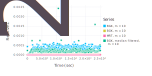
\includegraphics[width=\linewidth]{figs/poise-bingham/epsilon}
    \caption{Evolution of relative $L_2$, $\epsilon^{neq}$ with time. The norm of the $\epsilon^{neq}$ across the height of the channel is an indicator of an increase in oscillations at the lattice level due to the $\epsilon$ moment.}
    \label{fig:epsilon}
\end{figure}

\Fref{fig:qx} shows a measure of the nonequilibrium $q_x$ moment, or energy flux in the x-direction, with respect to time for each of the collision schemes and was calculated using:
\begin{equation}
    \frac{||\mathbf{q_x} - \mathbf{q_x}^{eq}||_2}{||\mathbf{q_x}^{eq}||_2}
\end{equation}
\noindent where $q_{x_j} = - 2f_1(\pos_j) + 2f_3(\pos_j) + f_5(\pos_j) - f_6(\pos_j) - f_7(\pos_j) + f_8(\pos_j)$ and $\pos_j$ were taken across the height of the channel in the same manner as with the $\epsilon$ moment.
The values measured for the BGK with $m = 10^8$ and median filtered were consistently greater than any other collision scheme.
The $q_x$ moment was likely the cause of the significant error and noise in the BGK with $m = 10^8$ and median filtering solution.
As expected, the $q_x^{neq}$ relative $L_2$ for the BGK with $m = 10^8$ was slightly greater than the BGK with $m = 10^5$, and the $q_x^{neq}$ relative $L_2$ was negligible for the MRT collision scheme.
These results are consistent with the solution noise and error.

\begin{figure}
	\centering
    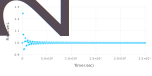
\includegraphics[width=\linewidth]{figs/poise-bingham/qx}
    \caption{Evolution of relative $L_2$, $q_x^{neq}$ with time. The norm of the $q_x^{neq}$ across the height of the channel is an indicator of an increase in oscillations at the lattice level due to the $q_x$ moment.}
    \label{fig:qx}
\end{figure}

It is likely that the nonequilibrium $\epsilon$ and $q_x$ moment cause oscillations at the lattice level that have a cumulative effect in time.
\Fref{fig:epsilon-cumulative} and \Fref{fig:qx-cumulative} show the cumulative measures of the nonequilibrium moments in time.
\Fref{fig:qx-cumulative} suggests that the $q_x^{neq}$ dominates and is the primary source of oscillations.
If an LBM collision scheme is to be developed for simulating high yield stress flows that is more accurate than the BGK with $m = 10^5$ and more computationally efficient than the MRT, it should focus on a means of dampening the nonequilibrium energy flux moments, namely $q_x$ and $q_y$.

\begin{figure}
    \includegraphics[width=\linewidth]{figs/poise-bingham/epsilon_cumulative}
    \caption{Cumulative relative $L_2$, $\epsilon^{neq}$ with time. Oscillations can have a positive effect on each other, building up. The cumulative relative $L_2$, $\epsilon^{neq}$ is a measure of how much oscillations due to the $\epsilon$ moment may have been building in time.}
    \label{fig:epsilon-cumulative}
\end{figure}

\begin{figure}
    \includegraphics[width=\linewidth]{figs/poise-bingham/qx_cumulative}
    \caption{Cumulative relative $L_2$, $q_x^{neq}$ with time. Oscillations can have a positive effect on each other, building up. The cumulative relative $L_2$, $q_x^{neq}$ is a measure of how much oscillations due to the $q_x$ moment may have been building in time.}
    \label{fig:qx-cumulative}
\end{figure}

\subsubsection{Power-law Fluids} \label{sec:poise-powerlaw}

The power-law simulations were carried out with a pressure gradient of $\pgrad = 1.0 \times 10^{-5}$, and a flow consistency index of $k = 0.2$.
The flow behavior index was varied between the four different values $n = [0.5, 0.75, 1.25, 1.50]$, and four different LBM schemes were used: (1) BGK, (2) BGK with median filtering, (3) MRT, and (4) BGK-BRT, with $\omega$ bounded within $[0.05, 1.995]$. 
The relative $L_2$ and relative $L_{\infty}$ errors with respect to the analytical solution were computed for each simulation.
The analytical solution for power-law fluid flow is given by:
\begin{equation} \label{eq:analytical-power-law}
  u_x(y) = \frac{n}{n+1}\left(-\frac{1}{k}\pgrad\right)^{1/n}\left[h^{\frac{n+1}{n}} - |y|^{\frac{n+1}{n}}\right].
\end{equation}

The results are presented in \Fref{tab:poise-power-law}.
In reference to computational time, each of the simulations in this section were run on a single core of an Intel I7-860 Quad-Core 2.80GHz processor.
The Reynold's number was computed by $Re = \frac{\rho U^{2-n} H^n}{k}$, where $U$ is the maximum velocity given by the analytical solution and $H = 2h$ is the total height of the channel.

% MG: it might be better to normalize the time with respect to the fastest, BGK with no filtering

\begin{table}
\centering
\caption{Power-law Poiseuille flow}
\vspace{0.5cm}
\begin{tabulary}{\linewidth}{l l r r r r r}
\pbox{20cm}{Collision \\ Operator} & \pbox{20cm}{Median \\ Filter} & $n$ & $Re$ & $L_2$ & $L_\infty$ & \pbox{20cm}{Time \\ (sec)} \\
\hline \\
BGK & No & 0.50 & 0.0007 & 28.06 & 30.37 & 5232 \\
& & 0.75 & 0.9125 & 0.0328 & 0.0569 & 2399 \\
& & 1.25 & 423.2 & 0.0051 & 0.0055 & 2311 \\
& & 1.50 & 2213 & 1.0 & 1.0 & 3622 \\
\\
BGK & Yes & 0.50 & 0.0007 & 26.72 & 28.78 & 5347 \\
& & 0.75 & 0.9125 & 0.0328 & 0.0569 & 2385 \\
& & 1.25 & 423.2 & 0.0051 & 0.0055 & 2275 \\
& & 1.50 & 2213 & 0.0570 & 0.0600 & 2357 \\
\\
MRT & No & 0.50 & 0.0007 & 0.1758 & 0.1401 & 4906 \\
& & 0.75 & 0.9125 & 0.0058 & 0.0045 & 4880 \\
& & 1.25 & 423.2 & 0.0051 & 0.0055 & 4863 \\
& & 1.50 & 2213 & 1.0 & 1.0 & 15992 \\
\\
BGK-BRT & No & 0.50 & 0.0007 & 11.73 & 12.56 & 4450 \\
& & 0.75 & 0.9125 & 0.0320 & 0.0475 & 1805 \\
& & 1.25 & 423.2 & 0.0051 & 0.0055 & 1905 \\
& & 1.50 & 2213 & 1.0 & 1.0 & 8194 \\
\\
\label{tab:poise-power-law}
\end{tabulary}
\end{table}

There are some interesting things to note from the power-law Poiseuille flow results.
Although for $n = 0.5, 0.75, 1.25$ there is still the same efficiency for accuracy trade off when it comes to deciding between the BGK and MRT collision operators, for $n = 1.5$ the BGK operator with median filtering was the fastest, most accurate, and only solution that remained stable.
In fact, besides for the case of $n = 0.5$, i.e. rather extreme shear-thinning, the BGK with median filtering was both fast and accurate.
The BGK-BRT had a moderate improvement of accuracy and efficiency--with respect to the regular BGK collision scheme--for flows where the constitutive relationship was only somewhat nonlinear, i.e. for $n = 0.75, 1.25$.
Note that none of the collision schemes were sufficiently accurate for the case of $n = 0.5$, and to improve this accuracy it would be necessary for a modeler to use a different simulation Mach number, a finer grid, and/or a smaller pressure gradient.

\subsection{Lid-driven Cavity Flow} % MG: would it be of any use to show streamline plots from some of these flows?

Lid-driven cavity flow is another good benchmark for two-dimensional fluid flow because it is sufficiently simple in terms of boundary conditions and implementation, while also complex in the flows and vortices it produces.
The lid-driven benchmark was chosen for this numerical study because there are many results available in literature in which to compare with and because the vorticity of the flow coupled with the nonlinear constitutive equations should result in a challenge in terms of stability.
Lid-driven cavity flow is generally characterized by a square cavity where a fluid velocity is prescribed tangential to the upper boundary and the remaining boundaries have a no-slip boundary condition.
Lid-driven cavity flow is depicted in \Fref{fig:lid-driven}.

\begin{figure}
\centering
\includegraphics{figs/lid-driven}
\caption{Schematic of lid-driven cavity flow; a velocity is prescribed tangential to the top boundary and no-slip is enforced at the remaining boundaries.}
\label{fig:lid-driven}
\end{figure}

The lid-driven cavity simulations presented in the section were all simulated on a coarse, $100 \times 100$ lattice; a coarse lattice was chosen in order to highlight concerns with stability and accuracy.
The simulations were run for either 50000 timesteps, or until convergence was met.
Convergence was defined by,
\begin{equation} \label{eq:convergence}
\sum_{m=1}^{100} \sum_{i, j} \frac{|u_{i, j}^k - u_{i, j}^{k-m}|}{|u_{i, j}^{k-m}|} < 1.0 \times 10^{-7},
\end{equation}
\noindent where $i$ is the node index in the x-direction, $j$ is the node index in the y-direction, and $k$ is the current timestep.
In reference to computational time, each of the simulations in this section were run on a single core of either an Intel I7-860 Quad-Core 2.80GHz processor, or an Intel Xeon v2 2.60 GHz processor.
The lid velocity was prescribed at $u_o = 0.1$.
For the MRT relaxation matrix, the free parameters were set to $s_1 = 1.1$, $s_2 = 1.0$, and $s_4 = s_6 = 1.2$.
All coordinate values presented in this section (used to describe the location of the center of vortices) are given normalized with respect to the length of the cavity side, i.e. as $(x / L, y / L)$.
Note that all results presented as ``-'' indicate that the tests were numerically unstable to the extent that the degrees of freedom all over the domain were ``NaN''.

\subsubsection{Bingham Plastic Fluids}

For the Bingham plastic numerical tests the Reynold's number was varied, $Re = 100, 1000, 5000, 1000$, and the Bingham number was varied, $Bn = 1, 10, 100$ ($Bn$ and $Re$ were calculated the same as in \Fref{sec:poise-bing}).
The collision schemes that were tested were: (1) BGK with $m = 10^5$, (2) BGK with $m = 10^8$, (3) BGK-BRT with $m = 10^8$, (4) BGK with $m = 10^8$ and median filtering, (5) MRT with $m = 10^8$ and (6) MRT with $m = 10^8$ and median filtering.
Tables \ref{tab:lid-bing1}--\ref{tab:lid-bing100} compare the center location of the main vortex to literature values taken from~\citet{syrakos2014performance}.
The main vortex location is determined by calculating the stream function using Simpson's rule and finding where it attains a maximum.

\begin{table}
\centering
\caption{Bingham plastic, lid-driven cavity flow; $Bn = 1$.}
\small
\vspace{0.5cm}
\begin{tabulary}{\linewidth}{r r l l r r r r}
$Bn$ & $Re$ & \pbox{20cm}{Collision \\ Operator} & \pbox{20cm}{Median \\ Filter} & $m$ & \pbox{20cm}{Vortex \\ Center \\ (literature)} &  \pbox{20cm}{Vortex \\ Center \\ (LBM)} & \pbox{20cm}{Time \\ (sec)} \\
\hline \\
1 & 100 & BGK     & No  & $10^5$ & (0.63, 0.79) & (0.63, 0.79) & 17685 \\
  &     & BGK     & No  & $10^8$ &              & (0.63, 0.79) & 19398 \\
  &     & BGK-BRT & No  & $10^8$ &              & (0.63, 0.79) & 22656 \\
  &     & BGK     & Yes & $10^8$ &              & (0.63, 0.79) & 21535 \\
  &     & MRT     & No  & $10^8$ &              & (0.63, 0.79) & 79040 \\
  &     & MRT     & Yes & $10^8$ &              & (0.63, 0.79) & 85295 \\
\\
1 & 1000 & BGK     & No  & $10^5$ & (0.54, 0.57) & (0.54, 0.57) & 16109 \\
  &      & BGK     & No  & $10^8$ &              & (0.54, 0.57) & 17035 \\
  &      & BGK-BRT & No  & $10^8$ &              & (0.54, 0.57) & 16879 \\
  &      & BGK     & Yes & $10^8$ &              & (0.54, 0.57) & 20170 \\
  &      & MRT     & No  & $10^8$ &              & (0.54, 0.57) & 46048 \\
  &      & MRT     & Yes & $10^8$ &              & (0.54, 0.57) & 55818 \\
\\
1 & 5000 & BGK     & No  & $10^5$ & (0.52, 0.53) & - & - \\
  &      & BGK     & No  & $10^8$ &              & - & - \\
  &      & BGK-BRT & No  & $10^8$ &              & - & - \\
  &      & BGK     & Yes & $10^8$ &              & (0.54, 0.53) & 17248 \\
  &      & MRT     & No  & $10^8$ &              & (0.51, 0.55) & 50572 \\
  &      & MRT     & Yes & $10^8$ &              & (0.52, 0.53) & 54225 \\
\\
1 & 10000 & BGK     & No  & $10^5$ & N/A          & - & - \\
  &       & BGK     & No  & $10^8$ &              & - & - \\
  &       & BGK-BRT & No  & $10^8$ &              & - & - \\
  &       & BGK     & Yes & $10^8$ &              & (0.56, 0.60) & 18186 \\
  &       & MRT     & No  & $10^8$ &              & (0.48, 0.48) & 43246 \\
  &       & MRT     & Yes & $10^8$ &              & (0.46, 0.54) & 50864 \\
\\
\end{tabulary}
\label{tab:lid-bing1}
\end{table}
\begin{table}
\centering
    \caption{Bingham plastic, lid-driven cavity flow; $Bn = 10$.}
    \small
    \vspace{0.5cm}
\begin{tabulary}{\linewidth}{r r l l r r r r}
    $Bn$ & $Re$ & \pbox{20cm}{Collision \\ Operator} & \pbox{20cm}{Median \\ Filter} & $m$ & \pbox{20cm}{Vortex \\ Center \\ (literature)} &  \pbox{20cm}{Vortex \\ Center \\ (LBM)} & \pbox{20cm}{Time \\ (sec)} \\
    \hline \\
10 & 100 & BGK     & No  & $10^5$ & (0.53, 0.87) & (0.54, 0.87) & 25217 \\
   &     & BGK     & No  & $10^8$ &              & (0.55, 0.87) & 38285 \\
   &     & BGK-BRT & No  & $10^8$ &              & (0.55, 0.87) & 29539 \\
   &     & BGK     & Yes & $10^8$ &              & (0.54, 0.87) & 35817 \\
   &     & MRT     & No  & $10^8$ &              & (0.53, 0.88) & 143741 \\
   &     & MRT     & Yes & $10^8$ &              & (0.54, 0.88) & 135059 \\
\\
10 & 1000 & BGK     & No  & $10^5$ & (0.80, 0.85) & (0.78, 0.83) & 11525 \\
   &      & BGK     & No  & $10^8$ &              & (0.78, 0.83) & 26671 \\
   &      & BGK-BRT & No  & $10^8$ &              & (0.78, 0.83) & 19248 \\
   &      & BGK     & Yes & $10^8$ &              & (0.79, 0.84) & 34143 \\
   &      & MRT     & No  & $10^8$ &              & (0.79, 0.84) & 105136 \\
   &      & MRT     & Yes & $10^8$ &              & (0.79, 0.84) & 111942 \\
\\
10 & 5000 & BGK     & No  & $10^5$ & (0.60, 0.55) & - & - \\
   &      & BGK     & No  & $10^8$ &              & - & - \\
   &      & BGK-BRT & No  & $10^8$ &              & - & - \\
   &      & BGK     & Yes & $10^8$ &              & (0.52, 0.55) & 34638 \\
   &      & MRT     & No  & $10^8$ &              & (0.55, 0.55) & 111274 \\
   &      & MRT     & Yes & $10^8$ &              & (0.55, 0.53) & 121685 \\
\\
10 & 10000 & BGK     & No  & $10^5$ & N/A          & - & - \\
   &       & BGK     & No  & $10^8$ &              & - & - \\
   &       & BGK-BRT & No  & $10^8$ &              & - & - \\
   &       & BGK     & Yes & $10^8$ &              & (0.49, 0.54) & 19351 \\
   &       & MRT     & No  & $10^8$ &              & (0.53, 0.54) & 69249 \\
   &       & MRT     & Yes & $10^8$ &              & (0.53, 0.53) & 69054 \\
\\
\end{tabulary}
\label{tab:lid-bing10}
\end{table}
\begin{table}
\centering
    \caption{Bingham plastic, lid-driven cavity flow; $Bn = 100$.}
    \small
    \vspace{0.5cm}
    \begin{tabulary}{\linewidth}{r r l l r r r r}
        $Bn$ & $Re$ & \pbox{20cm}{Collision \\ Operator} & \pbox{20cm}{Median \\ Filter} & $m$ & \pbox{20cm}{Vortex \\ Center \\ (literature)} &  \pbox{20cm}{Vortex \\ Center \\ (LBM)} & \pbox{20cm}{Time \\ (sec)} \\
        \hline \\
100 & 100 & BGK     & No  & $10^5$ & (0.51, 0.95) & (0.51, 0.95) & 13237 \\
    &     & BGK     & No  & $10^8$ &              & (0.54, 0.96) & 26782 \\
    &     & BGK-BRT & No  & $10^8$ &              & (0.53, 0.96) & 33095 \\
    &     & BGK     & Yes & $10^8$ &              & (0.58, 0.96) & 34430 \\
    &     & MRT     & No  & $10^8$ &              & (0.49, 0.95) & 161998 \\
    &     & MRT     & Yes & $10^8$ &              & (0.54, 0.96) & 162085 \\
\\
100 & 1000 & BGK     & No  & $10^5$ & (0.53, 0.95) & (0.54, 0.95) & 42233 \\
    &      & BGK     & No  & $10^8$ &              & (0.64, 0.95) & 47364 \\
    &      & BGK-BRT & No  & $10^8$ &              & (0.60, 0.92) & 46289 \\
    &      & BGK     & Yes & $10^8$ &              & (0.79, 0.95) & 48225 \\
    &      & MRT     & No  & $10^8$ &              & (0.54, 0.95) & 190119 \\
    &      & MRT     & Yes & $10^8$ &              & (0.55, 0.95) & 188242 \\
\\
100 & 5000 & BGK     & No  & $10^5$ & (0.93, 0.97) & - & - \\
    &      & BGK     & No  & $10^8$ &              & - & - \\
    &      & BGK-BRT & No  & $10^8$ &              & - & - \\
    &      & BGK     & Yes & $10^8$ &              & (0.91, 0.95) & 57354 \\
    &      & MRT     & No  & $10^8$ &              & (0.92, 0.96) & 163318 \\
    &      & MRT     & Yes & $10^8$ &              & (0.93, 0.95) & 159523 \\
\\
100 & 10000 & BGK     & No  & $10^5$ & (0.92, 0.94) & - & - \\
    &       & BGK     & No  & $10^8$ &              & - & - \\
    &       & BGK-BRT & No  & $10^8$ &              & - & - \\
    &       & BGK     & Yes & $10^8$ &              & (0.84, 0.88) & 32080 \\
    &       & MRT     & No  & $10^8$ &              & (0.89, 0.91) & 152707 \\
    &       & MRT     & Yes & $10^8$ &              & (0.89, 0.91) & 145722 \\
\\
\end{tabulary}
\label{tab:lid-bing100}
\end{table}

Just as before with the Bingham plastic Poiseuille flow, if a modeler is using the BGK collision operator and entropic filtering is not available, a stress growth exponent of $m = 10^5$ yields faster, more accurate results (assuming the literature values are a good measure of accuracy) than using a larger stress growth exponent.
A smaller stress growth exponent is also more effective at producing accurate results in the BGK collision scheme than placing bounds on the relaxation time (BGK-BRT).
However, although the BGK with $m = 10^5$ was the fastest model in all cases, it was also--like the other two BGK models without median filtering--unstable for $Re \ge 5000$.

For flows with $Re \ge 5000$, the BGK with $m = 10^8$ and median filtering produced numerically stable results, but did not always seem to be consistent with literature values.
The apparent inaccuracy with regards to BGK with $m = 10^8$ and median filtering is probably due to how the numerical stability is enhanced--namely through artificial, nonphysical dissipation.
In contrast to the nonphysical nature in which median filtering enhances stability, the stability enhancement used by MRT does not directly affect the macroscopic hydrodynamics of interest, so it again provides a stable, and typically, the most accurate solution. % MG: verify this sentence is correct
The apparent superiority in terms of stability and accuracy of the MRT collision operator still comes at a price though.
The MRT collision operator was, in general, 5-10 times slower than any of the BGK collision schemes.
The extreme increase in computational expense is probably not due to the collision process itself, i.e. \eqref{eq:mrt-colop}, but instead calculating the strain-rate \eqref{eq:srtensor-mrt} for each iteration of the solution for $\mu_{app}$.

For the sake of completeness, the MRT collision operator was also tested with median filtering applied.
There does not seem to be any reason to recommend the MRT collision operator with median filtering in practice because the MRT collision operator is stable all on its own and the artificial dissipation introduced by median filtering has the potential to adversely affect the accuracy of the results.

In summary, 
\begin{itemize}
    \item for low Reynold's number flows when computational efficiency is important, the BGK with $m = 10^5$ is recommended,
    \item for high Reynold's number flows when computational efficiency is important, the BGK with $m = 10^8$ and median filtering is recommended,
    \item and for high Reynold's number flows when accuracy is more important than computational efficiency, the MRT with $m = 10^8$ is recommended.
\end{itemize} 

\subsubsection{Power-law Fluids}

For the power-law numerical tests the Reynold's number was varied, $Re = 100, 1000, 5000, 1000$, and the flow behavior index was varied, $n = 0.5, 1.5$ ($Re$ was calculated the same as in \Fref{sec:poise-powerlaw}).
The collision schemes that were tested were: (1) BGK, (2) BGK-BRT, (3) BGK with median filtering, (4) MRT with $m = 10^8$ and (5) MRT with $m = 10^8$ and median filtering.
\Fref{tab:lid-powerlaw05} and \Fref{tab:lid-powerlaw15} compare the center location of the main vortex to literature values taken from~\citet{li2014simulation}.
The main vortex location is determined by calculating the stream function using Simpson's rule and finding where it attains a maximum.

%MG: two values still need filled in in these tables
\begin{table}
\centering
\caption{Power-law, lid-driven cavity flow; $n = 0.5$.}
\small
\vspace{0.5cm}
\begin{tabulary}{\linewidth}{r r l l r r r}
$n$ & $Re$ & \pbox{20cm}{Collision \\ Operator} & \pbox{20cm}{Median \\ Filter} & \pbox{20cm}{Vortex \\ Center \\ (literature)} &  \pbox{20cm}{Vortex \\ Center \\ (LBM)} & \pbox{20cm}{Time \\ (sec)} \\
\hline \\
0.5 & 100 & BGK     & No  & (0.72, 0.78) & (0.71, 0.77) & 21429 \\
    &     & BGK-BRT & No  &              & (0.71, 0.77) & 14547 \\
    &     & BGK     & Yes &              & (0.72, 0.78) & 33221 \\
    &     & MRT     & No  &              & (0.71, 0.77) & 77287 \\
    &     & MRT     & Yes &              & (0.71, 0.77) & 110403 \\
\\
0.5 & 1000 & BGK     & No  & (0.58, 0.55) & - & - \\
    &      & BGK-BRT & No  &              & - & - \\
    &      & BGK     & Yes &              & (0.53, 0.59) & 24935 \\
    &      & MRT     & No  &              & (0.53, 0.54) & 72102 \\
    &      & MRT     & Yes &              & (0.53, 0.54) & 78300 \\
\\
0.5 & 5000 & BGK     & No  & (0.53, 0.52) & - & - \\
    &      & BGK-BRT & No  &              & - & - \\
    &      & BGK     & Yes &              & (0.63, 0.68) & 23517 \\
    &      & MRT     & No  &              &              &       \\
    &      & MRT     & Yes &              & (0.51, 0.58) & 54225 \\
\\
0.5 & 10000 & BGK     & No  & (0.53, 0.52) & - & - \\
    &       & BGK-BRT & No  &              & - & - \\
    &       & BGK     & Yes &              & (0.50, 0.55) & 22603 \\
    &       & MRT     & No  &              &              &       \\
    &       & MRT     & Yes &              & (0.50, 0.54) & 63892 \\
\\
\end{tabulary}
\label{tab:lid-powerlaw05}
\end{table}

\begin{table}
\centering
\caption{Power-law, lid-driven cavity flow; $n = 1.5$.}
\small
\vspace{0.5cm}
\begin{tabulary}{\linewidth}{r r l l r r r}
$n$ & $Re$ & \pbox{20cm}{Collision \\ Operator} & \pbox{20cm}{Median \\ Filter} & \pbox{20cm}{Vortex \\ Center \\ (literature)} &  \pbox{20cm}{Vortex \\ Center \\ (LBM)} & \pbox{20cm}{Time \\ (sec)} \\
\hline \\
1.5 & 100 & BGK     & No  & (0.56, 0.73) & (0.57, 0.73) & 10897 \\
    &     & BGK-BRT & No  &              & (0.57, 0.73) & 6239 \\
    &     & BGK     & Yes &              & (0.56, 0.73) & 11847 \\
    &     & MRT     & No  &              & (0.56, 0.73) & 39017 \\
    &     & MRT     & Yes &              & (0.56, 0.73) & 96033 \\
\\
  1.5 & 1000 & BGK   & No  & (0.55, 0.64) & (0.54, 0.61) & 19764 \\
    &      & BGK-BRT & No  &                & (0.54, 0.61) & 11949 \\
    &      & BGK     & Yes &                & (0.54, 0.61) & 24516 \\
    &      & MRT     & No  &                & (0.54, 0.61) & 58714 \\
    &      & MRT     & Yes &                & (0.54, 0.61) & 69884 \\
\\
  1.5 & 5000 & BGK     & No  & (0.53, 0.61) & (0.52, 0.57) & 20147 \\
    &      & BGK-BRT & No  &              & (0.52, 0.57) & 12116 \\
    &      & BGK     & Yes &              & (0.52, 0.57) & 23140 \\
    &      & MRT     & No  &              & (0.53, 0.57) & 60584 \\
    &      & MRT     & Yes &              & (0.52, 0.58) & 58519 \\
\\
  1.5 & 10000 & BGK     & No  & (0.51, 0.55) & (0.53, 0.55) & 21570 \\
    &       & BGK-BRT & No  &              & (0.53, 0.55) & 12841 \\
    &       & BGK     & Yes &              & (0.53, 0.55) & 21570 \\
    &       & MRT     & No  &              & (0.49, 0.56) & 61453 \\
    &       & MRT     & Yes &              & (0.49, 0.55) & 67546 \\
\\
\end{tabulary}
\label{tab:lid-powerlaw15}
\end{table}

For the shear-thinning results, $n = 0.5$, the BGK and BGK-BRT collision schemes were unstable when $Re \ge 1000$.
Although there still appears to be somewhat of a trade off between computational efficiency and accuracy in regards to the BGK with median filtering and MRT collision schemes, it does not seem to be nearly as drastic as when simulating Bingham plastic lid-driven flow; e.g. neither collision scheme consistently agrees with the literature values; and the MRT collision operator is only 2-3 times slower than the BGK with median filtering.

For the shear-thickening results, $n = 1.5$, there are no issues of stability.
What is interesting is that all of the collision schemes produce similar results for each of the cases (with the exception of the high Reynold's number case, $Re = 10000$), and the BGK-BRT is consistently the fastest solution.
The reason the BGK-BRT may be the fastest is that because the collision frequency, $\omega$, is bounded, and consequently $\mu_{app}$ is bounded, meaning the solution to the constitutive equation may be converging to a bound with less iterations than the other collision schemes.

In summary, 
\begin{itemize}
    \item for shear-thinning flows, either the BGK with median filtering or MRT collision schemes are recommended for stability reasons,
    \item for shear-thickening flows, there is much less concern for numerical instability.
\end{itemize}

\section{Conclusion}

A numerical investigation into the accuracy, stability, and efficiency of LBM collision models when applied to non-Newtonian flows was presented.
The numerical investigation included testing the BGK and MRT collision operators, with and without entropic filtering, as applied to Bingham plastics and power-law fluid flows.
Two different benchmark problems were chosen for the flows: Poiseuille flow, and lid-driven square cavity flow.
The results showed that:
\begin{itemize}
  \item For high yield stress fluids in Poiseuille-type flows, only the MRT collision operator did not suffer from numerical noise.
  \begin{itemize}
      \item The noise appeared to be due to oscillations arising from high nonequilibrium values for the moment related to the square of the energy, $\epsilon$, and the energy flux moment in the direction of flow, $q_x$.
      \item If a collision scheme is to be developed for high yield stress, Poiseuille-type flows that is more accurate than the BGK with $m = 10^5$ and more computationally efficient than the MRT, then it should focus on dampening the nonequilibrium energy flux moment.
    \end{itemize}
  \item Median filtering can be an effective technique for enhancing stability, especially for high Reynold's number flows; however, if the filter is not carefully tuned by properly adjusted the threshold, $\delta$, or number of standard deviations, $n_s$, then the physical intregrity, and consquently accuracy, of the model can be adversely impacted.
  \item In general, the MRT collision operator is much more computationally expensive than its BGK counterpart and is some times even orders of magnitude slower.
  \item To summarize plastic, lid-driven cavity flows,
    \begin{itemize}
  \item for low Reynold's number flows when computational efficiency is important, the BGK with $m = 10^5$ is recommended,
  \item for high Reynold's number flows when computational efficiency is important, the BGK with $m = 10^8$ and median filtering is recommended,
  \item and for high Reynold's number flows when accuracy is more important than computational efficiency, the MRT with $m = 10^8$ is recommended.
    \end{itemize}
  \item To summarize power-law, lid-driven cavity flows,
    \begin{itemize}
  \item for shear-thinning either the BGK with median filtering or MRT collision schemes are recommended for stability reasons,
  \item for shear-thickening, lid-driven cavity flows, there is much less concern for numerical instability.
    \end{itemize}
\end{itemize}

% MG: should we mention: code is open source? input files used in this study are also freely available?

\chapter{Free Surface and non-Newtonian Simulation of Wellbore Cementing using the Lattice Boltzmann Method} \label{chap:lbm-cement}

\section*{Abstract}

When oil and gas wellbores are drilled, barriers must be put in place to ensure that fluids do not leak out of the wellbore.
Wellbore leakage can lead to environmental damage, loss of pressure at the wellhead, and consequently, loss of production.
An important yet vulnerable barrier is the cement annulus.
Creating the cement annulus, a process known as primary cementing, is difficult to perform optimally.
Every well has unique subsurface conditions, and so no cement slurry mix design both performs well and is economical for all wells.
Although some general guidelines and analytical techniques exist for approximating the performance of a cement slurry mix, the mechanics of primary cementing are complex.
Computational methods can help better understand primary cementing and aid designers in determining the optimal mix.
The lattice Boltzmann method (LBM) is a promising technique for simulating primary cementing because it is well-suited for efficiently simulating non-Newtonian flows, multiphase multicomponent flows, and flows through complex geometries--namely, some of the complexities associated with the mechanics of primary cementing.
In \Fref{sec:numerical-methods}, an algorithm for simulating non-Newtonian free-surface flow using LBM is presented.
The algorithm was implemented and used to study primary cementing of a dry annulus, i.e. an annulus that is not filled with drilling mud.
More specifically, the study involved parameterizing different cement slurry flows and investigating how well each slurry flow filled different wellbore geometries.
The study is followed by conclusions and a discussion of future work.

\section{Introduction}

% what is primary cementing?

Of critical importance to drilling operations of all kinds is that barriers are placed to prevent gasses and fluids from migrating from one geological zone to another (i.e., zonal isolation is achieved).
If zonal isolation is not achieved, gasses and fluids may migrate through the well to the surface and up into the atmosphere--potentially causing pollution, or at the very least, contributing to an increase in greenhouse gasses--or, worse yet, formation gasses and fluids can migrate into aquifers, potentially harming wild life and people.
Furthermore, it can be argued that the most important, yet vulnerable, barrier in terms of achieving zonal isolation of a wellbore is the cement annulus that is created between the casing and the formation.
There are various mechanisms by which this cement annulus can fail.
According to previous studies~\cite{Bit02,Che85,Lev79,Ste88,Tal93,Zul12}, the most prevalent failure mechanisms of the cement annulus are:
\begin{itemize}
\item Stresses developing in the cement annulus as a result of temperature gradients, moisture gradients, overburden pressure, and chemical shrinkage of the cement matrix.
These stresses can cause cracking in the cement, or debonding at either the casing--cement or cement--formation interfaces.
\item Poor fill of the annulus. If cement slurry does not fill the annulus then if drilling mud is left behind it can dry, crack, and provide a weak path for fluids and gasses under pressure to push through, or if a dry hole is is cemented and not filled properly, fluids and gasses can travel through channels and voids left in the annular space.
\item Gas channeling through the annulus during cement curing.
Initially, after the annulus is poured, the cement column transmits its full hydrostatic pressure against the rock formation.
As the cement annulus hydrates, it solidifies, becoming stiffer and more self-supporting.
When the column begins to support itself, the hydrostatic pressure of the cement column--against the rock formation--begins to drop.
If the hydrostatic pressure of the cement column drops below the pressure of a formation gas before the cement annulus has developed adequate strength to resist it, the formation gas can penetrate int the cement annulus and form channels, or degrade the cement annulus in other ways.
\end{itemize}
% what research has been done that is considered classical?

% why do we need modelling?
% Before the end of this paragraph--modeling is important because...

In order to better understand, and thus improve primary cementing for zonal isolation, several works have attempted to model certain aspects of the multiphase and multiphysics processes of wellbore cement placement.
For example,~\citet{Bei77} developed a mathematical model to ``describe the miscible displacement of drilling muds by cement slurries under laminar flow conditions''.
Among their assumptions were that the process could be modeled in a quasi-steady manner, the volumetric flow rate was constant at each cross section of the flow, and the pressure fields were only dependent on the y-coordinate.
The model was then used to explore the effect of various parameters on the displacement efficiency of the spacer, such as the density ratio between the mud and the spacer, the viscosity ratio between the mud and the spacer, the displacement rate, the displaced phase yield stress, and the displacing phase yield stress.
It was concluded that displacement efficiency could be improved by increasing the density of the displacing phase, increasing the viscosity of the displacing phase, (in general) decreasing the displacement rate, decreasing the yield stress of the displaced phase, and increasing the yield stress of the displacing phase.
\citet{Bit02} developed a mathematical model for primary cementing of an oil well using a Hele-Shaw displacement model.
The model was more general than the model developed by~\citeauthor{Bei77} as it used less restrictive assumptions and was able to consider an eccentric annulus.
Annulus eccentricity occurs often in wellbores and can sometimes be extreme as it is difficult to keep long strings of casing centered in an imperfectly drilled hole.
The bulk fluid motion of the spacer and drilling mud during primary cementing were investigated.
The intended use of the model was not to make general statements about what properties of the spacer and drilling mud were desirable, but to instead be used iteratively during the design process for the cement job.
Results showed that the model met its intended purpose, and in particular, was able to simulate an unyielded channel of mud left on the narrow side of the annulus.
\citet{Zul12} used a computational fluids dynamics (CFD) solver with volume of fluid (VOF) method to simulate the cementing process of a 50 ft. section of wellbore.
The model included the interfacial dynamics of, not just the spacer and drilling mud, but also the cement slurry--which was not considered in either~\citeauthor{Bei77} or~\citeauthor{Bit02}.
The drilling mud and cement slurry properties were kept constant, while the spacer density, viscosity, and displacement rates were varied.
\citeauthor{Zul12} concluded that the high displacement efficiency occurred when the spacer was the same density as the drilling mud and had a smaller viscosity, similar to that of water.
The displacement efficiency was poor for all scenarios in which the spacer and cement slurry densities were equal.
\citet{zhao2016lattice} developed a model simulating primary cementing using the Lattice Boltzmann Method.
\citeauthor{zhao2016lattice} used the model to investigate the displacement interface shape in a horizontal, eccentric annulus; and in order to simplify the model from a 3D to 2D flow, used the classical Hele-Shaw approach.
It was found, in general, that a greater density ratio between the displacing phase, i.e. cement slurry, and displaced phase, i.e. drilling mud, and lower eccentricity, results in better displacement in a horizontal, eccentric annulus.

% talk about new LBM study

Overall, past studies have tended to idealize the rock formation as a straight wall.
Although this is a desirable simplification to make for capturing bulk fluid phenomena, it does not accurately describe what is happening locally at the surface of the rock formation.
Flow near the surface of the formation, and in and around the imperfections of the formation geometry, could influence the bond of the cement annulus to the rock formation, and the fill of the cement slurry very near to the rock formation.
If an adequate bond does not develop, debonding can occur as a result of thermal and mechanical stresses.
Even if most of the annulus is filled by the cement slurry, a small gap at the cement--formation interface that stretches for a long enough span of the wellbore would still be susceptible to fluid and gas migration, i.e. loss of zonal isolation.
One could even argue that the characteristic of the cement slurry flow is most important local to the cement--formation interface, and that considering imperfections in the rock formation is imperative to determining whether zonal isolation has been achieved.

The purpose of the current work is to develop a computational approach to investigate the flow of cement slurry in and around the--possibly--imperfect features of a rock formation in a vertical section of a wellbore, with the hope of better understanding what parameters of the primary cement job will lead to a good fill of the cement annulus and high bond strength at imperfect rock formation features (i.e., the purpose of the current work is an extension of the work present in~\citet{grasinger2015simulation}).
The Lattice Boltzmann Method (LBM) was chosen as the most suitable modeling technique for the desired purpose because of its ability to model flow through and around complex geometries~\cite{thorne2006lattice}, such as those found at the surface of the rock formation, among other benefits.
LBM also has other advantages as an approach for simulating primary cementing:
\begin{itemize}
\item LBM is well-suited for simulating non-Newtonian fluids because the strain-rate tensor is computed local to each node and is second-order accurate~\cite{kruger2009shear,kruger2010second}.
Many fluids present in primary cementing such as the spacer, drilling mud, and most importantly, the cement slurry, are best modeled as non-Newtonian fluids.
\item LBM is well-suited for simulating multiphase multicomponent flows and free-surface flows because it can handle complicated interface shapes between fluid phases and components.
\item LBM is easily written in parallel.
As hardware architectures shift from one or a few cores to, especially in the case of scientific computing, several CPUs, it becomes increasingly important that code for simulating complex and computationally expense phenomena be written in parallel.
\end{itemize}
The current work focuses on the problem of cementing a dry hole, i.e. an annulus that is not filled with drilling mud prior to cementing.
In order to numerically investigate this problem, an LBM model for non-Newtonian and free-surface flow is developed.
The details of the LBM model are outlined in \Fref{sec:numerical-methods}.
What follows in \Fref{sec:results} is a preliminary study on how different characteristics of flow, e.g. cement slurry yield stress, cement slurry inlet velocity, etc., perform in regards to fill of the annulus for different wellbores with imperfect rock formation geometries.
\Fref{sec:conclusion} outlines conclusions resulting from the numerical study and a discussion of future work.

\section{Numerical Methods} \label{sec:numerical-methods}

\subsection{Lattice Boltzmann Method}

% We need to explain/justify why 2D vs. 3D

For the sake of computational simplicity and computational efficiency, the numerical study considered a two-dimensional section of the wellbore and was simulated using the D2Q9 lattice.
In addition, the collision operator used was the BGK collision operator.
For more details on the Lattice Boltzmann Method, the D2Q9 lattice, or the BGK collision operator, see \Fref{sec:LBM}.

\subsection{Cement Slurry Constitutive Relationship}

Cement slurry is best modeled using a non-Newtonian constitutive relationship.
A simple, yet accurate constitutive relationship for cement slurry is the Bingham plastic constitutive relationship.
Bingham plastics are characterized by a plastic viscosity, which is analogous to the dynamic viscosity for Newtonian fluids, and a yield stress, which is a stress threshold that, if the shear stress does not exceed, the strain-rate is zero.
The Bingham plastic constitutive model is difficult to work with numerically.
Often, a smooth approximation is used instead--the Papastasiou approximation.
Throughout this chapter, the Papastasiou approximation with a stress growth exponent of $m = 10^6$ is used.
The BGK collision operator with $m = 10^6$ can be seen as a compromise between computational efficiency and accuracy for simulating Bingham plastic flows.
For more detail on Bingham plastics or the Papastasiou approximation, see \Fref{sec:bp}.

\subsection{Free Surface Flow}

A free-surface flow is a flow in which two-fluids exist but the dynamics of one fluid does not need to be explicitly modeled.
Typically, the phase of the primary fluid, or the fluid of interest, is a liquid; and the secondary phase that does not need to be explicitly modeled is a gas, often times air at atmospheric pressure.
The primary fluid is modeled using a standard CFD method, such as LBM, and the interaction of the secondary fluid on the primary fluid is modeled as a boundary condition at the interface between the two fluids.
The interface is what is referred to as the free-surface.
The advantage of modeling a multiphase multicomponent flow as a free-surface is that, because the dynamics of the secondary fluid are not explicitly tracked and simulated, the resulting algorithm is more computationally efficient in terms of both memory and CPU overhead.
The algorithm for extending the Lattice Boltzmann Method for free-surface flow used in this work follows the algorithm developed and presented in~\citet{korner2005lattice,thurey2005interactive}.

\subsection{Capturing the Free-Surface}

Consider at each node a cell of size $\text{d}x \times \text{d}x$ where $\text{d}x$ is the distance between nodes and the cell is centered at the node.
In order to track where the primary fluid is and where it is not, i.e. which cells contain the primary fluid, a variable is introduced, $\epsilon$, which describes what fraction of the cell is covered by the primary fluid.
Cells that have a fluid fraction of $\epsilon = 0$ contain no primary fluid, i.e. are empty; cells that have a fluid fraction of $\epsilon = 1$ are filled; and cells that have a fluid fraction $0 < \epsilon < 1$ are neither completely filled nor are they completely empty.
The fluid fraction concept is similar to how fluids are tracked in Volume of Fluid (VOF) methods.

\subsubsection{Mass Transfer}

It is important to note that the particle distributions, $f_0, ..., f_8$, cannot be used to directly determine the fluid fraction of a cell.
Neither can the zeroth velocity moment of the particle distributions, $\rho = \sum_i f_i$.
For the algorithm used in this work, $\epsilon(\pos, t) \neq \epsilon(\mathbf{f(\pos, t)}, \rho(\pos, t))$.
Instead, each $f_i$ is related to the amount of primary fluid advection in each of the $\pvel_i$ discrete velocity directions.
To track the fluid fraction and how it changes, another variable is introduced, $M(\pos, t)$, which denotes the (primary) fluid mass in each cell.
The fluid mass is related to the fluid fraction by $\epsilon = M / \rho$.
The change in mass, $\Delta M(\pos, t)$ is related to $\mathbf{f}(\pos, t)$ and particle distribution in the neighborhood of $\pos$.
Given initial conditions on $M(\pos, 0)$ and a fixed time step size $\Delta t $, the fluid mass is determined by $M(\pos, t_n) = M(\pos, 0) + \Delta t \sum_{k=1}^n \Delta M(\pos, t_k)$.
What remains to track the fluid mass is to develop an expression for $\Delta M(\pos, t)$.

\newcommand{\opidx}{{\bar{i}}}
\newcommand{\fset}{\mathcal{F}}
\newcommand{\iset}{\mathcal{I}}
\newcommand{\gset}{\mathcal{G}}
\newcommand{\domain}{\mathcal{X}}

\subsubsection{Cell States} \label{sec:mass-transfer}

Each of the cells in the domain are assigned one of three states: fluid, interface, or gas.
The set of fluid, interface, and gas cells are denoted by $\fset$, $\iset$, and $\gset$, respectively.
A fluid cell is a cell that is entirely covered by the primary fluid; and a gas cell is a cell that is completely empty, or does not contain any primary fluid.
An interface is partially covered, and there is always a layer of interface cells between fluid and gas cells so that a fluid cell and a gas cell are never neighbors.
The change in mass is calculated across fluid and interface cells for each discrete velocity direction as follows:
\begin{equation} \label{eq:dM}
\Delta M_i(\pos, t) = \begin{cases}
f_\opidx(\pos + \pvel_i \Delta t, t) - f_i(\pos, t), & \pos \in \fset \text{ or } \pos + \pvel_i \in \fset \\
\left[(\epsilon(\pos, t) + \epsilon(\pos + \pvel_i \Delta t, t)) / 2\right]\left(f_\opidx(\pos + \pvel_i, t) - f_i(\pos, t)\right), & \pos \in \iset \text{ and } \pos + \pvel_i \in \iset \\
0, & \pos + \pvel_i \in \gset
\end{cases}
\end{equation}
\noindent where $\pvel_\opidx$ represents the discrete velocity vector that is opposite in direction to $\pvel_i$, i.e. $\pvel_\opidx = - \pvel_i$.
\eqref{eq:dM} states that when the border of the two cells is covered with fluid, the change in mass for a discrete velocity direction is equal to the difference of the particle distribution entering the cell from the opposite direction and particle distribution leaving the cell in that direction.
When the border of the two cells are not covered with fluid, i.e. when both cells are interface cells, the difference is weighted by the average fluid fraction of the two cells because mass is only able to transfer across the fraction of the cell border that is covered in fluid.
The total change in mass for a cell is simply $\Delta M(\pos, t) = \sum_i \Delta M(\pos, t)$.
Finally, note that $\Delta M_i(\pos, t) = -\Delta M_\opidx(\pos + \pvel_i \Delta t, t)$ for all $\pos \in \domain$ where $\domain$ is the domain.
As a consequence, it is clear that $\sum_{\pos \in \domain}\Delta M(\pos, t) = 0$, i.e. that mass is conserved for the mass transfer step.

\newcommand{\tconst}{\delta_{trans}}

Tracking the transport of mass throughout the domain is an important step in determining what parts of the domain contain the primary fluid and what do not.
However, for the free-surface to change shape and propagate, cells need to be able to transition state.
Cell states change based on the rule set presented in \Fref{tab:cell-transition-rules} where $\tconst$ is a small, computational constant that keeps cells from transitioning back and forth between fluid and interface, or interface and gas states in subsequent time steps.
To summarize \Fref{tab:cell-transition-rules}, gas cells cannot transition to fluid cells and vice versa, interface cells transition to fluid cells when their mass has exceeded $\rho$ by a computational constant, and gas cells when their mass is less than zero minus a computational constant.
In addition, fluid cells and gas cells transition to the interface state in order to maintain continuity of the interface, i.e. to ensure there is always a layer of interface cells in between fluid cells and gas cells.
An example of a cell transitioning state is depicted in \Fref{fig:cell-transition}.

\begin{table}
\caption{Cell state transition rules.}
\begin{tabulary}{\linewidth}{l|L|L}
\textbf{Current State} & \textbf{Condition} & \textbf{Transition} \\
\hline &  & \\
$(\pos, t) \in \iset$ & $M(\pos, t) < -\tconst$ & $(\pos, t + \Delta t) \rightarrow \gset$, $M(\pos, t + \Delta t) = 0$ \\
                      & $M(\pos, t) > \tconst + \rho(\pos, t)$ & $(\pos, t + \Delta t) \rightarrow \fset$, $M(\pos, t + \Delta t) = \rho(\pos, t + \Delta t)$ \\
                      &\\
$(\pos, t) \in \fset$ & $(\pos + \pvel_i \Delta t, t + \Delta t) \in \gset$ for any $i = 1, 2, ..., 8$ & $(\pos, t + \Delta t) \rightarrow \iset$ \\
&\\
$(\pos, t) \in \gset$ & $(\pos + \pvel_i \Delta t, t + \Delta t) \in \fset$ for any $i = 1, 2, ..., 8$ & $(\pos, t + \Delta t) \rightarrow \iset$ \\
\end{tabulary}
\label{tab:cell-transition-rules}
\end{table}

\begin{figure}
\centering
\includegraphics{figs/cell-transition}
\caption{Example of cell state transitions.
The interface cell highlighted in red on the left is transitioned to a gas cell as it has emptied.
On the right, the three cells highlighted in red were transitioned from fluid to interface cells in order to keep the interface continuous.}
\label{fig:cell-transition}
\end{figure}

\subsubsection{Updating Cell States and Mass Redistribution} \label{sec:cell-updates}

The rules for updating cell states in \Fref{tab:cell-transition-rules} are fairly intuitive, however, there are some bookkeeping nuances that must be considered in order to ensure mass is properly conserved and interface continuity is achieved; e.g. note that if the rules outlined in \Fref{tab:cell-transition-rules} are followed naively that mass is not conserved when interface cells transition to fluid cells or gas cells.
The algorithm for updating cell states follows that which was presented in~\citet{thurey2005interactive}.
It is presented here for the sake of completeness and for outlining minor modifications.
\begin{enumerate}
\item Initialize a variable that represents the global excess mass, e.g. $M_{gex} = 0$.
\item For all cells $\pos \in \iset$, store cells that should be transitioned to $\fset$ in one data structure, $\iset_f$, and store cells that should be transitioned to $\gset$ in another, $\iset_g$.
\item \label{enum:prep-fnbrs} Loop over cells that will be transitioned from interface to fluid cells, i.e. loop over $\iset_f$, and prepare their neighborhoods for transition:
	\begin{enumerate}
	\item Calculate the average density, $\rho_{avg}$, and velocity, $\mathbf{u}_{avg}$, of each neighborhood.
	\item For all cells in the neighborhood of the new fluid cell:
		\begin{enumerate}
			\item If the cell is a gas cell, transition to interface state and set $f_i = f_i^{eq}(\rho_{avg}, \mathbf{u}_{avg})$, $\rho = \rho_{avg}$, and $\mathbf{u} = \mathbf{u}_{avg}$.
			\item If the cell is an interface cell in $\iset_g$, remove it from $\iset_g$.
		\end{enumerate}
	\end{enumerate}
\item \label{enum:prep-gnbrs} Loop over cells that will be transitioned from interface to gas cells, i.e. loop over $\iset_g$, and prepare their neighborhoods for transition:
	\begin{enumerate}
	\item For all cells in the neighborhood of the new gas cell:
		\begin{enumerate}
			\item If the cell is a fluid cell, transition to interface state.
		\end{enumerate}
	\end{enumerate}
\item \label{enum:rloop-fluid} Loop over cells that will be transitioned from interface to fluid cells, i.e. loop over $\pos \in \iset_f$, and:
\begin{enumerate}
	\item Let $M_{ex} = M - \rho$.
	\item Calculate the unit norm outward from the interface, i.e. toward empty space, $\mathbf{n}$.
	Initialize $v_{sum} = 0$.
	\item For all cells in the neighborhood,
	\begin{enumerate}
		\item if an interface cell, store in a data structure, $\iset_{r}$, and for the discrete velocity vector direction, $\pvel_i$, of the respective neighbor, let $v_i = \begin{cases}
					\mathbf{n} \cdot \pvel_i, & \mathbf{n} \cdot \pvel_i > 0 \\
					0, & \text{otherwise}
				\end{cases}$.
		\item $v_{sum} = v_{sum} + v_i$.
	\end{enumerate}
	\item If $v_{sum} \ge 0$, then for each cell, $\pos_j \in \iset_r$, redistribute the excess mass according to $M(\pos_j) = M(\pos_j) + M_{ex} \frac{v_i}{v_{sum}}$. \label{enum:redist-dop-f}
	\item \label{enum:redist-neighbors-f} If $v_{sum} = 0$ and $\iset_r \neq \emptyset$, then for each cell, $\pos_j \in \iset_r$, redistributed the excess mass according to $M(\pos_j) = M(\pos_j) +  M_{ex} / n_r$ where $n_r$ is the number of cells in $\iset_r$.
	\item Otherwise, increment the global excess mass, $M_{gex} = M_{gex} + M_{ex}$.
	\item Lastly, transition $\pos$ from $\iset$ to $\fset$ and $M(\pos) = \rho(\pos)$.
\end{enumerate}
\item \label{enum:rloop-gas} Loop over cells that will be transitioned from interface to gas cells, i.e. loop over $\pos \in \iset_g$, and:
\begin{enumerate}
	\item Let $M_{ex} = M$.
	\item Calculate the unit norm outward from the interface, i.e. toward empty space, $\mathbf{n}$.
	Initialize $v_{sum} = 0$.
	\item For all cells in the neighborhood,
	\begin{enumerate}
		\item if an interface cell, store in a data structure, $\iset_{r}$, and for the discrete velocity vector direction, $\pvel_i$, of the respective neighbor, let $v_i = \begin{cases}
					-\mathbf{n} \cdot \pvel_i, & \mathbf{n} \cdot \pvel_i < 0 \\
					0, & \text{otherwise}
				\end{cases}$.
		\item $v_{sum} = v_{sum} + v_i$.
	\end{enumerate}
	\item \label{enum:redist-dop-g} If $v_{sum} \ge 0$ and $\iset_r \neq \emptyset$, then for each cell, $\pos_j \in \iset_r$, redistribute the excess mass according to $M(\pos_j) = M(\pos_j) +  M_{ex} \frac{v_i}{v_{sum}}$.
	\item \label{enum:redist-neighbors-g} If $v_{sum} = 0$ and $\iset \neq \emptyset$, then for each cell, $\pos_j \in \iset_r$, redistributed the excess mass according to $M(\pos_j) = M(\pos_j) + M_{ex} / n_r$ where $n_r$ is the number of cells in $\iset_r$.
	\item Otherwise, increment the global excess mass, $M_{gex} = M_{gex} + M_{ex}$.
	\item Lastly, transition $\pos$ from $\iset$ to $\gset$ and $M(\pos) = 0$.
\end{enumerate}
\item \label{enum:final-redist} The global excess mass, i.e. the mass that could not be redistributed by other means, is redistributed according to:
\begin{enumerate}
	\item \label{enum:final-rloop} for all $\pos \in \iset$, $M(\pos) = M(\pos) + M_{gex} / n_i$ where $n_i$ is equal to the number of cells in the interface set, $\iset$.
\end{enumerate}
\end{enumerate}
The algorithm, as presented, ensures both mass conservation and continuity of the free-surface.
Moreover, when mass redistribution inevitably occurs, it is first attempted to be redistributed and weighted in the direction in which the interface is propagating, e.g. as in Step \ref{enum:rloop-fluid}.\ref{enum:redist-dop-f} or \ref{enum:rloop-gas}.\ref{enum:redist-dop-g}.
If there are no interface cells in the direction of interface propagation, it is instead redistributed to neighboring interface cells, e.g. Step \ref{enum:rloop-fluid}.\ref{enum:redist-neighbors-f} or \ref{enum:rloop-gas}.\ref{enum:redist-neighbors-g}.
On the off-chance that there are no neighboring cells which are interface cells, the excess mass is added onto the global excess mass, $M_{gex}$, which is eventually redistributed among all of the interface cells, e.g. Step \ref{enum:final-redist}.
The hierarchy of possible redistribution steps ensures that mass redistribution is done in the most physically meaningful way as is possible. % We may need to hard code references to steps in here...
Lastly, note that the interface normal, $\mathbf{n}$, is calculated using a finite difference approximation,
\begin{equation} \label{eq:n}
\mathbf{n}_{ij} = \frac{1}{2} \begin{Bmatrix}
\epsilon_{i-1, j} - \epsilon_{i+1, j} \\
\epsilon_{i, j-1} - \epsilon_{i, j+1}
\end{Bmatrix}
\end{equation}
\noindent where $i$ is the index of the node in the x-direction and $j$ is the index of the node in the y-direction.

\subsection{Boundary Conditions at the Free-Surface} \label{sec:bc-at-fs}

Two important considerations not yet discussed are how boundary conditions are implemented at the interface in order to capture the interaction between the primary phase and the secondary phase, and a still more subtle consideration, how particle distributions that are missing from the streaming step are reconstructed.
The degrees of freedom, $f_i$, are not tracked for gas cells.
After the streaming step, interface cells will be missing particle distributions that would have streamed from gas cells--an issue that is depicted in \Fref{fig:ps}.

\begin{figure}
\centering
\includegraphics{figs/ps}
\caption{Example of a scenario in which particle distributions are missing post-streaming.}
\label{fig:ps}
\end{figure}

The missing particle distributions need reconstructed.
Also momentum needs to be conserved at the interface.
When the particle distributions are reconstructed, they will be reconstructed in such a way that momentum is conserved between the primary fluid and the secondary fluid.
In order to perform the reconstruction, there are a few assumptions that need to be made:
\begin{enumerate}
\item The velocity of the secondary fluid is equal to the velocity of the primary fluid at the free-surface, i.e. there is no-slip between the two-fluids.
\item The secondary fluid is at equilibrium and at constant pressure, $p_G$.
\item There is a force balance for opposite lattice directions.
\end{enumerate}
Because particle distributions are a measure of momentum transport, the pressure of the secondary fluid can be converted to the particle distribution scale and the missing particle distribution can be solved for algebraically.
Consider \Fref{fig:fbi}.
Balancing the opposite lattice directions results in:
\begin{eqnarray}
f_i + f_\opidx &=& f^{eq}_\opidx(\rho_G, \mathbf{u}) + f_i^{eq}(\rho_G, \mathbf{u}), \\
\label{eq:reconst} f_\opidx &=& f_\opidx^{eq}(\rho_G, \mathbf{u}) + f_i^{eq}(\rho_G, \mathbf{u}) - f_i.
\end{eqnarray}
Missing distribution functions can be reconstructed according to \eqref{eq:reconst}.
In order for conservation of momentum to be satisfied along the free-surface, distribution functions coming from the direction of the interface normal, $\mathbf{n}$, must also be reconstructed.
Thus, distribution functions are reconstructed if coming from a gas cell, or if $\mathbf{n} \cdot \pvel_\opidx > 0$.

\begin{figure}
\centering
\includegraphics{figs/force-bal-at-interface}
\caption{Particle distributions at free-surface for a pair of opposing lattice directions after gas pressure, $\rho_G$, is in the particle distribution form.}
\label{fig:fbi}
\end{figure}

\subsection{Resulting Algorithm}

The details of the free-surface algorithm have not been presented in chronological order, but instead in a logical order.
For reasons of clarity, the steps of the algorithm are presented in order:
\begin{enumerate}
\item Mass transfer (\Fref{sec:mass-transfer})
\item Stream
\item Reconstruct particle distributions (\Fref{sec:bc-at-fs})
\item Collide
\item Enforce boundary conditions
\item Calculate macroscopic variables
\item Update cell states (\Fref{sec:cell-updates})
\end{enumerate}

\newcommand{\nodesi}{50}
\newcommand{\nodesj}{500}
\newcommand{\anw}{$1\frac{1}{4}$"}
\newcommand{\anh}{1'}
\newcommand{\nsteps}{16000}

\section{Primary Cementing} \label{sec:results}

The free-surface LBM model was implemented and used to simulate primary cementing in a dry annulus, i.e. an annulus without drilling mud.
The focus of the current study was the performance of different cement slurry mixes and characteristic flows when used to cement different imperfect wellbore geometries.
Because the focus in regards to the wellbore is on geometrical imperfections, the entire wellbore annulus is not simulated, but instead a small section around a geometrical imperfection is considered.
An example is shown in \Fref{fig:wellbore-cementing-schematic}.

\begin{figure}
\centering
\includegraphics{figs/wellbore-cementing-schematic}
\caption{Example simulation used in primary cementing study.
The black rectangles on the left boundary represent notches protruding from the rock formation surface. The contours are of the primary fluid (cement slurry) mass.}
\label{fig:wellbore-cementing-schematic}
\end{figure}

The simulations were carried out on a $\nodesi \times \nodesj$ lattice, which corresponds to an annulus width of \anw \hspace{0.05cm} and a sectional height of \anh.
For the mass inlet, a~\citet{zou1997pressure} velocity boundary condition was used in conjuction with a constant mass boundary condition, i.e. $M(\pos_i, t) = M_0 = 1.0$ for all $\pos_j$ along the inlet.
This corresponded to a constant mass flow, $\dot{M}_{in} = M_0 u_0$, at inlet.
For the outlet, mass was allowed to transfer out of the domain during the mass transfer step such that $f_\opidx(\pos + \pvel_i \Delta t, t) = 0$ in \eqref{eq:dM} for all $\pos + \pvel_i$ that lie outside of the domain on the other side of the mass outlet, i.e. the boundary condition at the outlet is such that there is no backflow.
All simulations were executed for \nsteps time steps.

Both the rock formation geometries and cement slurry flow properties were parameterized.
The different imperfect geometries that were considered at the rock formation surface were: flow over a cavity that is 30\% of the annulus width, ``cav $30 \times 1$''; flow over a cavity that is 60\% of the annulus width, ``cav $60 \times 1$''; flow over a square obstacle with sides that are 30\% of the annulus width, ``obs $30 \times 1$''; flow over two square obstacles with sides that are 30\% of the annulus width, ``obs $30 \times 2$''; flow over a square obstacle with sides that are 60\% of the annulus width, ``obs $60 \times 1$''; flow over two square obstacles with sides that are 60\% of the annulus width, ``obs $60 \times 2$''; and flow over a rectangular obstacle with width that is 60\% of the annulus width and length that is four times the width, ``obs $60 \times L$''.
The wellbore geometries are depicted in \Fref{fig:wellbore-geometries}.

\begin{figure}
\includegraphics[width=\linewidth]{figs/wellbore-geometries}
\caption{Wellbore geometries considered in the study.}
\label{fig:wellbore-geometries}
\end{figure}

In addition to wellbore geometry, different cement slurry material properties and cement slurry flow rates were parameterized, which are characterized by the dimensionless Reynold's number, $Re = \frac{\rho U L}{\mu_p}$, and Bingham number, $Bn = \frac{\tau_y L}{\mu_p U}$, of the flow where $L \equiv $ the width of the annulus.
The goal of the study was to investigate which Reynold's numbers and Bingham numbers were preferable for each geometry, and which Reynold's numbers and Bingham numbers performed well for all geometries.
The dimensionless numbers were parameterized as follows, $(Re, Bn) = (1.00, 4.00)$,  $(2.50, 0.00)$, $(2.50, 1.00)$, $(2.50, 10.0)$, $(2.50, 25.0)$, $(5.00, 5.00)$, and $(12.5, 2.0)$.
\Fref{fig:percent-filled} shows the percentage of the \anh \hspace{0.05cm} section wellbore filled after cementing.

\begin{figure}
\centering
\includegraphics[width=\linewidth]{figs/percent_filled}
\caption{Wellbore geometries considered in the study.}
\label{fig:percent-filled}
\end{figure}

\Fref{fig:percent-filled} shows that there are some general statements to be made about what properties of the cement slurry flow are preferable.
For example, low yield stress, i.e. low Bingham number flows, had good fill for every wellbore geometry considered.
In addition, the good performance of the $Re = 5.00, Bn = 5.00$ and $Re = 12.5, Bn = 2.0$ slurry flows suggests that a if the ratio of $Bn / Re$ is low, that the slurry flow will perform well for cementing a dry hole.
As $Bn / Re$ increases, it appears that, in certain cases and wellbore geometries, the slurry flow tends to perform worse.
What is interesting to note is that for slurry flows that performed poorly in some cases, there was a lack of consistency across wellbore geometries in terms of which slurry flow performed worse and which slurry flows performed better, which suggests that generalities cannot always be made and that computational methods are necessary for understanding and designing slurry mixes for real-life wellbores.

\section{Conclusion} \label{sec:conclusion}

An LBM model for simulating the non-Newtonnian and free-surface flows that occurs while cementing dry annuli in oil and gas wellbores was implemented and presented.
It was then used to study how different cement slurry flows, parameterized by different Reynold's numbers and Bingham numbers, would perform in different wellbore geometries.
It was found that in general, it is preferable that the yield stress and $Bn / Re$ ratio of the slurry flow be low.
However, beyond these considerations, it is not clear what slurry flow may be preferable for a given rock formation geometry.
The results suggest that computational methods are necessary for (a) better understanding the mechanics of primary cementing and (b) for designing a cement mix for a given wellbore.
It is a goal of the current work to identify a computational method for efficiently simulating cement slurry flow through a realistic wellbore so that optimization methods may be used to determine the optimal cement slurry flow for primary cementing.
The lattice Boltzmann method extended for simulating non-Newtonian and free-surface flows as presented in the current work has several properties that make it a good candidate for such a design framework:
\begin{itemize}
\item LBM is well-suited for simulating non-Newtonian fluids because the strain-rate tensor is computed local to each node and is second-order accurate~\cite{kruger2009shear,kruger2010second}.
\item LBM is well-suited for simulating multiphase multicomponent flows and free-surface flows because it can handle complicated interface shapes between fluid phases and components.
\item LBM is easily written in parallel and as hardware architectures shifts sequential to parallel computing, it becomes increasingly important that code for simulating complex and computationally expense phenomena be written in parallel.
\item The LBM no-slip boundary condition works well with complex geometries, such as those that occur in realistic rock formation surfaces in drilled wellbores.
\end{itemize}

\bibliographystyle{abbrvnat}
\bibliography{master}
	
\end{document}
